\documentclass[11pt]{article}
\usepackage{geometry}                % See geometry.pdf to learn the layout options. There are lots.
\geometry{letterpaper}                   % ... or a4paper or a5paper or ... 
%\geometry{landscape}                % Activate for for rotated page geometry
%\usepackage[parfill]{parskip}    % Activate to begin paragraphs with an empty line rather than an indent
\usepackage{graphicx}
\usepackage{amssymb}
\usepackage{slashed}
\usepackage{epstopdf}
\usepackage{amsmath}
\DeclareGraphicsRule{.tif}{png}{.png}{`convert #1 `dirname #1`/`basename #1 .tif`.png}

\setlength{\parindent}{0pt}

\usepackage{lmodern}

\usepackage{mmacells}



\graphicspath{ {Scalar_figures/} }


\newcommand{\newc}{\newcommand}
\newcommand{\mychi}{\raisebox{0pt}[1ex][1ex]{$\chi$}}
\def\sp{\slashed{p}}
\def\sk{\slashed{k}}
\def\cn{\chi^0}
\def\cp{\chi^+}
\def\cm{\chi^-}
\def\gm{\gamma^{\mu}}
\def\gn{\gamma^{\nu}}
\def\gp{\gamma^{\rho}}
\def\km{k_{\mu}}
\def\kn{k_{\nu}}
\def\kp{k_{\rho}}
\renewcommand{\d}{\ensuremath{\operatorname{d}\!}}
\newc{\cTarasov}{a}


\def\cpp{\mychi^{++}}
\def\cmm{\mychi^{--}}
\def\Mp{M_{\text{pole}}}
\def\Mpa{M_{\text{pole},A}}
\def\Mpb{M_{\text{pole},B}}
\def\kmpm{k^{\mu}p_{\mu}}
\def\he{\frac{\epsilon}{2}}

\newcommand{\mb}{\textsf{Mass Builder} \! }
\newcommand{\tsil}{\textsf{TSIL} \! }
\newcommand{\tarcer}{\textsf{TARCER} \! }

%\title{Minimal dark matter self energy}


\begin{document}
%\maketitle
\section{Two-loop self energy calculations}

\subsection{Introduction}

In this document we present a self-contained calculation of the radiatively induced mass correction up to two-loop order in the perturbative couplings.  For the purposes of a fully self contained and explanatory presentation, we work through a simple scalar field theory example first using all the tools available.  This is followed by the more complicated electroweak triplet model, for which we are interested in obtaining the two-loop mass corrections to study the mass splittings between the triplet states.

define self energy for scalar, fermion and bosons.

introduce \mb and the related tools.


\subsection{Definitions}

We will make use of tools and literature sources which use slightly different definitions for the same mathematical objects.  In this section we make it clear what these differences are and how these differences alter the important relationships between these objects.


In the following I use bold-face for the divergent integrals and normal type for the finite pieces, as defined in the TSIL manual.  I use $\tt{TAI}$ to refer to TARCER notation and $A$ for TSIL notation as there is a different normalisation between such integrals.  We define $\kappa = 1/16\pi^2$.

We begin with $B_0$ and $B_1$.  These are defined by Ibe at al. as
\begin{eqnarray}
B_0(p^2, m_1^2, m_2^2) &=& \Delta
- \int_0^1 dx ~\log \frac{ (1-x)m_1^2 + x m_2^2 - x(1-x)p^2 -i\epsilon }{Q^2}\ , \\
B_1(p^2, m_1^2, m_2^2) &=& -\frac{\Delta}{2}
+ \int_0^1 dx ~x\log \frac{ (1-x)m_1^2 + x m_2^2 - x(1-x)p^2 -i\epsilon }{Q^2}\ , \\
B_{21}(p^2, m_1^2, m_2^2) &=& \frac{\Delta}{3}
- \int_0^1 dx ~x^2\log \frac{ (1-x)m_1^2 + x m_2^2 - x(1-x)p^2 -i\epsilon }{Q^2}\ ,
\end{eqnarray}

while BMPZ defines these as
\begin{eqnarray}
A_0(m) &=& 16\pi^2Q^{4-n}\int{d^nq\over i\,(2\pi)^n}{1\over
q^2-m^2+i\varepsilon}\\
B_0(p, m_1, m_2) &=&
16\pi^2Q^{4-n}\int{d^nq\over i\,(2\pi)^n}
{1\over\biggl[q^2-m^2_1+i\varepsilon\biggr]\biggl[
(q-p)^2-m_2^2+i\varepsilon\biggr]}
\label{B0 def}  \\
p_\mu B_1(p, m_1,m_2) &=& 16\pi^2Q^{4-n}\int
{d^nq\over i\,(2\pi)^n}{q_\mu\over\biggl[q^2-m^2_1+i\varepsilon\biggr]
\biggl[(q-p)^2-m_2^2+i\varepsilon\biggr]}\label{B1 def} \\ p_\mu p_\nu
B_{21}(p,m_1,m_2) &+& g_{\mu\nu}B_{22}(p,m_1,m_2)
\label{B22 def}\\
 &=& 16\pi^2\,Q^{4-n}\,\int{d^nq\over i\,(2\pi)^n} {q_\mu
q_\nu\over\biggl[q^2-m^2_1+i\varepsilon\biggr]\biggl[
(q-p)^2-m_2^2+i\varepsilon\biggr]}\ , \nonumber
\end{eqnarray}
where we deal with $B_{22}$ later.  

The above definitions are not equivalent, first we need to set $\Delta = 2/(4-D)-\gamma_E+\log(4\pi)$ and $n=D$.  However, there is an important sign difference from the way the denominator is written.  BMPZ use $(p-k)$ while other sources, including Ibe et al. use $(p+k)$.  Therefore when doing the Feynman integration and introducing the step, we end up shifting the integration measure, $k$, by either $k+px$ or $k-px$.  This difference introduces a sign difference in the integrated form of $B_1$.  (need to check the validity of the relationship given in B.9 in BMPZ for the case of $(k+p)$.  \textcolor{red}{Therefore when we compare with the results stated in Ibe et al. we must be careful with the sign of the $B_1$ integral and make sure to introduce a negative.}
TSIL defines
\begin{eqnarray}
{\bf A}(x) &=&  
C \int d^d k \frac{1}{[k^2 +x]}  %,
\label{defineboldA}
\\
{\bf B}(x,y) &=&
C \int d^d k   \frac{1}{[k^2 +x] [(k-p)^2 +y]} .
\label{defineboldB}
\end{eqnarray}
where
\begin{equation}
C = (16 \pi^2) \frac{\mu^{2\epsilon}}{(2 \pi)^d}
  = (2 \pi \mu)^{2 \epsilon}/\pi^2 .
\end{equation}
and TARCER uses

\begin{eqnarray}
{\bf A}(x) &=& i \cTarasov \mbox{{\tt TAI$[$d,s,$\{\{1,\sqrt{x}\}\}]$}},
\\
{\bf B}(x,y) &=& -i \cTarasov \mbox{{\tt TBI$[$d,s,$\{%
\{1,\sqrt{x}\},\{1,\sqrt{y}\}\}]$}} 
\end{eqnarray}
where 
$
\cTarasov = (4 \pi \mu^2)^{2-d/2}.
$
So we make the identification that $n=D=4-2\epsilon$ and achieve equivalent pre-factors.  There is an important sign difference attached to the $m^2=x$ quantity between the different definitions of $A_0$ and $B_0$.  The effects the form of the finite plus divergent expansion of the basis integrals.  From the TSIL manual we have
\begin{eqnarray}
{\bf A}(x) &=& -x/\epsilon + A(x) + \epsilon A_\epsilon(x) + 
{\cal O}(\epsilon^2) 
\\
{\bf B}(x,y) &=& 1/\epsilon + B(x,y) + \epsilon B_\epsilon(x,y) 
+ {\cal O}(\epsilon^2) ,
\end{eqnarray}
so to make use of these with TARCER functions we must make the conversion to the form

\begin{eqnarray}
{\bf A}(x) &=& -x/\epsilon + A(x) + \epsilon A_\epsilon(x) + 
{\cal O}(\epsilon^2) 
\\
{\bf B}(x,y) &=& 1/\epsilon + B(x,y) + \epsilon B_\epsilon(x,y) 
+ {\cal O}(\epsilon^2) ,
\end{eqnarray}


So Ibe et al. do not define an $A_0$ function, instead using only $B_1$ which we can reduce down to a function of $B_0$ and $A_0$.  This relationship is essential for our calculations, and we will present it shortly.  First we need to draw a direct comparison between the above function definitions.


\subsection{Tensor integral reduction}

We need to compare self energies calculated with Mass Builder and those in the existing literature.  Comparing with Ibe et al. we need to understand the definitions used.

Ibe et al. make the following definitions:	

\begin{align}
\Pi_V &= -p^2 \left[ B_1(p^2,m_1^2,m_2^2)+B_{21}(p^2,m_1^2,m_2^2)\right]\\
\tilde{B}_{22}(p^2,m_1^2,m_2^2)&= -p^2(B_1+B_{21})-\frac{p^2}{4}B_0-\frac{1}{4}(m_1^2-m_2^2)(B_0+2B_1)
\end{align}

so to compare with the self energies presented within we need to determine exactly what $B_{21}$ is.  This requires finding equivalent definitions elsewhere to properly understand what is going on here.

In general we find the statement

\begin{align}
B_{\mu\nu}&=g_{\mu\nu}B_{00}+p_{\mu}p_{\nu}B_{11}\\
&=g_{\mu\nu}B_{22}+p_{\mu}p_{\nu}B_{21}\\
\end{align}

using FeynCalc to reduce the following (note that in FeynCalc notation $B_{22}$ is denoated $B_{00}$)
 
\begin{mmaCell}[functionlocal=y]{Code}
B22 = PaVe[0, 0, {p^2}, {m1^2,m2^2}]
B22r = PaVeReduce[B22]
\end{mmaCell}

\begin{mmaCell}{Output}
A0[m2^2]/(2 (-1 + D)) + (m1^2 B0[p^2, m1^2, m2^2])/(-1 + D) + (
 m1^2 B1[p^2, m1^2, m2^2])/(2 (-1 + D)) - (m2^2 B1[p^2, m1^2, m2^2])/(
 2 (-1 + D)) + (p^2 B1[p^2, m1^2, m2^2])/(2 (-1 + D))
\end{mmaCell}
next we need to further reduce the $B_1$ functions using
\begin{mmaCell}[functionlocal=y]{Code}
B22r = 
B22r/.B1-> -(-A0[m1^2]+A0[m2^2]+(p^2+m1^2-m2^2)*B0))/(2 p^2)
\end{mmaCell} 
we then to extract the finite pieces of this integral so we may compare with other sources.

\begin{mmaCell}[functionlocal=y]{Code}
CAw1 = Coefficient[B22r, A0[m1^2]] /. D-> 4-2\[Epsilon]
CAw2 = Coefficient[B22r, A0[m2^2]] /. D-> 4-2\[Epsilon]
CBww = Coefficient[B22r, B0[p^2,m1^2,m2^2]] /. D-> 4-2\[Epsilon]
A1 = A0[m1^2] + (m1^2/\[Epsilon]);
A2 = A0[m1^2] + (m2^2/\[Epsilon]);
Bww = B0[p^2,m1^2,m2^2] + (1/\[Epsilon]);
B22finite = 
 Coefficient[CAw1*Aw1+CAw2*Aw2+CBww*Bww, \[Epsilon], 0]
\end{mmaCell}


we first want to check that this is consistent with the definition given in BMPZ (arXiv:hep-ph/9606211v3), which is

\begin{eqnarray}
B_{22}(p, m_1,m_2) &=& {1\over 6}\ \Bigg\{\,
{1\over2}\biggl(A_0(m_1)+A_0(m_2)\biggr)
+\left(m_1^2+m_2^2-{1\over2}p^2\right)B_0(p,m_1,m_2)\nonumber \\ &+&
\ {m_2^2-m_1^2\over2p^2}\ \biggl[\,A_0(m_2)-A_0(m_1)-(m_2^2-m_1^2)
B_0(p,m_1,m_2)\,\biggr] \nonumber\\ &+&\ m_1^2 + m_2^2
-{1\over3}p^2\,\Bigg\}~.
\end{eqnarray}

and we find that these expressions do indeed agree.  This confirms that the FeynCalc definition of $B_{00}$ does indeed agree with the alternative used in the literature which is $B_{22}$.\\

We now need to determine exactly what the notation used in Ibe et al. is.  From BMPZ we have
\begin{align}
 \tilde
B_{22}(p,m_1,m_2)= B_{22}(p,m_1,m_2) - {1\over4}A_0(m_1) -
{1\over4}A_0(m_2) \label{eqn:B22_BMPZ}
\end{align}
and from Ibe et al. we have
\begin{align}
{\tilde B}_{22}(p^2, m_1^2, m_2^2) &=
- p^2 (B_1 + B_{21}) - \frac{p^2}{4} B_0 - \frac{1}{4}(m_1^2 - m_2^2) (B_0 + 2B_1)\ . \label{eqn:B22_Ibe}
\end{align}

so we have one undefined term here, $B_{21}$.  This is given in Ibe et al. in it's integrated form but we want it in terms of reduced one-loop basis integrals.  So, to determine this we will make the assumption that (\ref{eqn:B22_BMPZ}) and (\ref{eqn:B22_Ibe}) are equivalent and determine an ansatz for $B_{21}$.  We will then confirm this ansatz by calculating equation (B.5) from Ibe et al. independently and determining what $B_{21}$ is.  Comparing equations (\ref{eqn:B22_BMPZ}) and (\ref{eqn:B22_Ibe}) we determine
\begin{align}
B_{21}(p^2, m_1^2, m_2^2)  = \frac{1}{18 p^2} \left( 6 (p^2-m_1^2)B_0(p^2, m_1^2, m_2^2) +6A_0(m_1^2)-6m_1^2+p^2\right)
\end{align}

Now we calculate the contribution of the electroweak triplet state to the W boson self energy to double check if this definition of $B_{21}$ is consistent.  Calculating the required amplitude using Mass Builder (and associated tools) we find
\begin{align}
\Pi_{WW}^{(\tilde{\chi})}(p^2) =
\frac{\hat{g}^2}{36\pi^2} \left( 3 (2M^2+p^2)B_0(p^2,M^2,M^2)-6A_0(M^2)+6M^2-p^2\right)
\end{align}
which is consistent with the Ibe at al. calculation
\begin{align}
\Pi_{WW}^{(\tilde{\chi})}(p^2) = &
\frac{\hat{g}^2}{2\pi^2}
\Pi_V(p^2, \hat{M}_2^2, \hat{M}_2^2)\\
=& \frac{\hat{g}^2}{2\pi^2} \left\{-p^2 \left[ B_1(p^2,m_1^2,m_2^2)+B_{21}(p^2,m_1^2,m_2^2)\right]\right\}
\end{align}
which after using $B_1 = -B_0/2$ (since $m_1=m_2$) we obtain a consistent result.


\section{Scalar field theory}

The field theory we will deal with here is that with Lagrangian
\begin{align}
\mathcal{L} = \frac{1}{2}(\partial_{\mu} s)^2-\frac{1}{2}m^2s^2-\frac{g}{3!}s^3-\frac{\lambda}{4!}s^4
\end{align}
where $m$ is the mass of the field and we have two couplings, $g$ and $\lambda$, for the cubic and quartic interactions respectively.  We now need to redefine the field in couplings in terms of renormalised parameters,

\begin{align}
s\rightarrow Z^{1/2}_ss, \ \ \ m^2\rightarrow\frac{1}{Z_s}(m^2+\delta m^2),  \ \ \ g\rightarrow \frac{1}{Z_s^{3/2}}(g+\delta_g), \ \ \ \lambda\rightarrow \frac{1}{Z_s^2}(\lambda+\delta\lambda)
\end{align}
such that the Lagrangian becomes
\begin{align}
\mathcal{L} = \mathcal{L}_{free}+\mathcal{L}_{interaction}
\end{align}
where
\begin{eqnarray}
&\mathcal{L}_{free} &=  \ \ \frac{1}{2}(\partial_{\mu} s)^2-\frac{1}{2}m^2s^2\\
&\mathcal{L}_{interaction} &= \ -\frac{g}{3!}s^3-\frac{\lambda}{4!}s^4  +\frac{1}{2}(Z_s-1)(\partial_{\mu} s)^2 -\frac{\delta m}{2}m^2s^2-\frac{\delta g}{3!}s^3-\frac{\delta \lambda}{4!}s^4
\end{eqnarray}

We can use the above interaction Lagrangian to determine the Feynman rules for each vertex interaction.  For the two-point propagator we have the tree-level counter-term with interaction coupling $i(Z_s-1)k^2-i\delta m$.  We will define $Z_s-1=\delta Z$.  The cubic and quartic interactions are simply $-i\delta g$ and $-i\delta \lambda$ respectively, with no momentum dependant part.  Finally, the scalar propagator is given by
\begin{align}
\frac{1}{p^2-m^2+i\epsilon}
\end{align}
where $\epsilon\ll 1$.





\section{One-loop self energy}

In this section we present the one-loop corrections to the scalar propagator.  There are two loop corrections and one counter-term correction at the one-loop order which are represented in Figure \ref{fig:1loop} top and bottom respectively.  Although these are easily written down by hand we use \mb to carry out the calculation and demonstrate where we need to account for sign differences between the computational tools we interface with.


\begin{figure}[h!]
\center
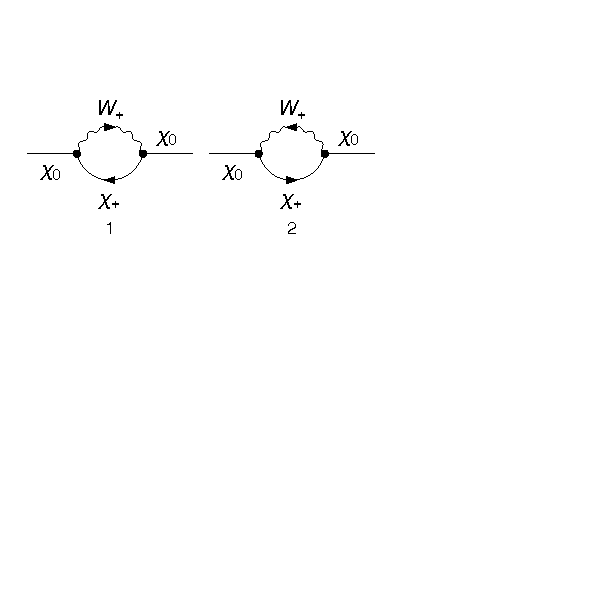
\includegraphics[width=0.6\textwidth]{1loop.pdf}\\
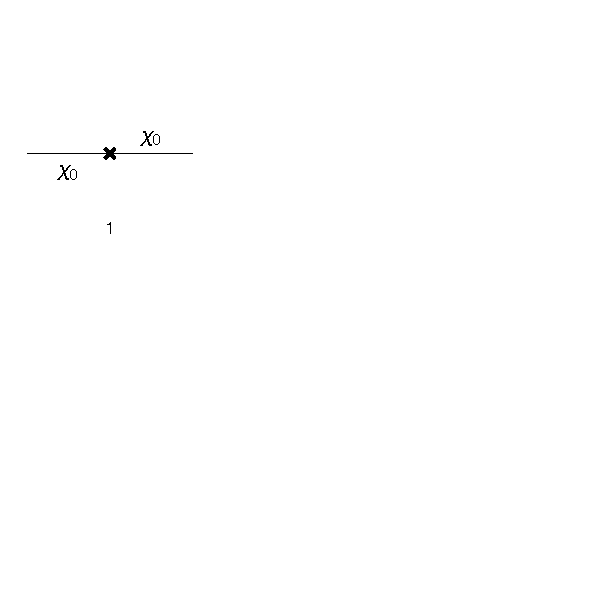
\includegraphics[width=0.3\textwidth]{1loop_1c.pdf}
\caption{The one-loop order loop (\textit{top}) and counter-term (\textit{bottom}) corrections to the scalar propagator.}\label{fig:1loop}
\end{figure}



The amplitudes from the loop corrections as output from \tarcer are
\begin{align}
\Pi^{(1)}_1 = -i \kappa \frac{\lambda}{2} \mathbf{TAI}(m^2)
\end{align}
and
\begin{align}
\Pi^{(1)}_2 =-i \kappa \frac{g^2}{2} \mathbf{TBI}(m^2,m^2)
\end{align}
first we must account for an overall negative sign in the amplitude, and then use the relationship $i\mathbf{TAI} = \mathbf{A}$ and $-i\mathbf{TBI} = \mathbf{B}$ to convert to \tsil notation
\begin{align}
\Pi^{(1)}_1 = \kappa \frac{\lambda}{2} \mathbf{A}(m^2)
\end{align}
and
\begin{align}
\Pi^{(1)}_2 = -\kappa \frac{g^2}{2} \mathbf{B}(m^2,m^2).
\end{align}

The counter-term diagram is trivial to calculate by hand, yet again we will take the result from \tarcer which is
\begin{align}
\Pi^{(1c)}_1 =  -\delta m + \delta Z p^2
\end{align}
so again we need to make a sign change and obtain
\begin{align}
\Pi^{(1c)}_1=  \delta m - \delta Z p^2
\end{align}


We can now determine this counter-term coupling from a simple calculation at one-loop, which we must do by hand.  The full one-loop self energy, including counter-terms, is
 \begin{align}
 \Pi_1 = \frac{1}{2}\kappa\lambda\left(A(m^2)+\epsilon A_{\epsilon}(m^2)-\frac{m^2}{\epsilon}\right)- \frac{1}{2}\kappa g^2\left(B(m^2)+\epsilon B_{\epsilon}(m^2)+\frac{1}{\epsilon}\right)+ \delta m - \delta Z p^2
 \end{align}
so the divergent part is
\begin{align}
\Pi_1^{1/\epsilon}=  -\frac{1}{2\epsilon}\kappa\left(\lambda m^2+g^2\right)+ \delta m - \delta Z p^2
\end{align}
so we find
\begin{eqnarray}
&\delta m &=\frac{\kappa}{2\epsilon} \left(g^2+\lambda m^2\right)+\mathcal{O}(\kappa^2)\\
&\delta Z &= 0
\end{eqnarray}
where we allow for high order terms which are required to cancel divergences from amplitudes above the one-loop order.  This counter-term is all we will need to compute the finite piece of the self energy at two-loop order under certain assumptions.

So at the one-loop level we make one sign change to the \tarcer output to be able to compute the self energy correctly via the \tsil integrals.

\section{Two-loop self energy}

There are 9 loop corrections and 5 counter-term corrections to the scalar propagator at the two-loop level.  We present the results as output by \tarcer and the required conversions to \tsil integrals on a diagram by diagram basis in this section.

\subsection*{Diagram 1}
\begin{center}
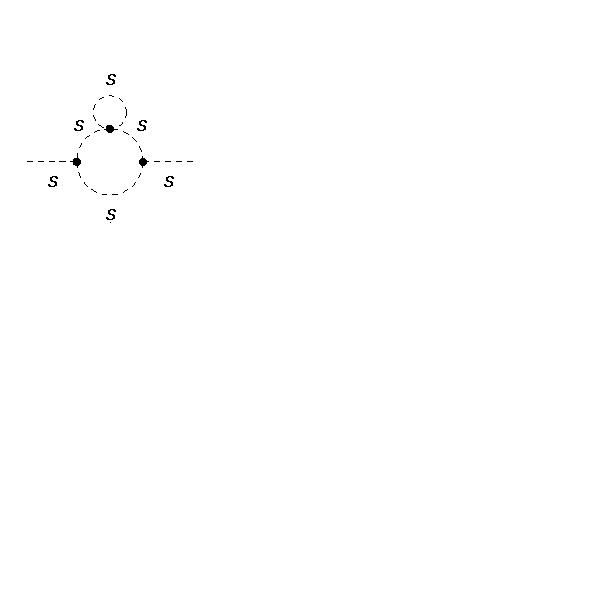
\includegraphics{2loop_1.pdf}\\
\end{center}
This digram is given by \tarcer to be
\begin{align}
\Pi^{(2)}_1 = \kappa^2\frac{g^2\lambda}{4} \frac{  \mathbf{TAI}(m^2) \left[ 2(D-3)m^2\mathbf{TBI}(m^2,m^2) - (D-2) \mathbf{TAI}(m^2) \right] }{m^2 (4m^2-p^2) }
\end{align}
so after accounting for the negative sign, and converting to TSIL notation (which also introduces a negative sign, due to the two factors of $i$) we obtain
\begin{align}
\Pi^{(2)}_1 = \kappa^2\frac{g^2\lambda}{4} \frac{  \mathbf{A}(m^2) \left[ -2(D-3)m^2\mathbf{B}(m^2,m^2) - (D-2) \mathbf{A}(m^2) \right] }{m^2 (4m^2-p^2) }
\end{align}


\subsection*{Diagram 2 and 3}
\begin{center}
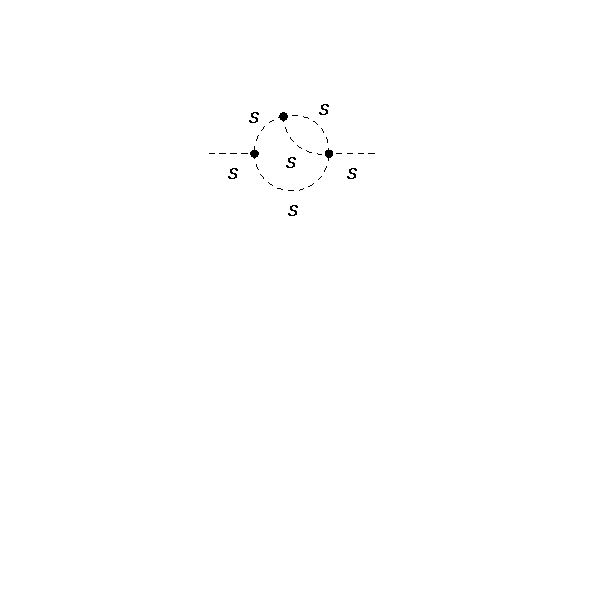
\includegraphics{2loop_2.pdf}\ \ \ \ \ \ 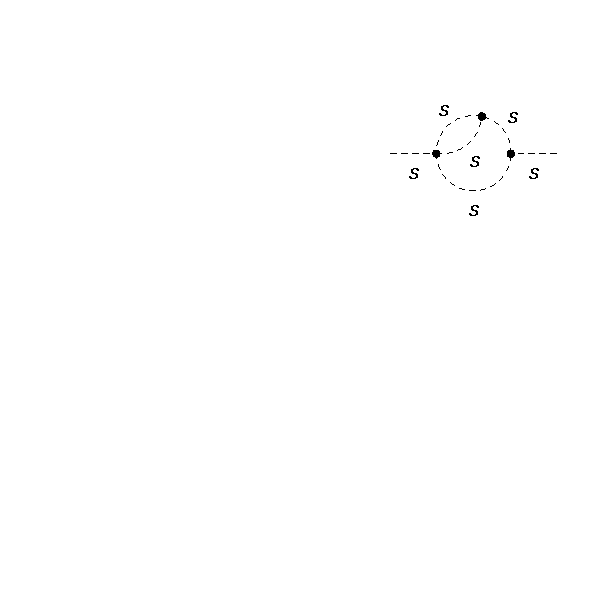
\includegraphics{2loop_3.pdf}\\
\end{center}
Diagrams 2 and 3 are identical and are given in \tarcer to be
\begin{align}
\Pi_2 = \kappa^2 \frac{g^2\lambda}{2} \mathbf{TVI}(m^2,m^2,m^2,m^2)
\end{align}
so combining these together and using the result $ \mathbf{TVI}=-\mathbf{U}$ we obtain, after including the sign change, the same result as we could get by simply looking at the topology of the diagram
\begin{align}
\Pi_2 =  \kappa^2 g^2\lambda \mathbf{U}(m^2,m^2,m^2,m^2).
\end{align}



\subsection*{Diagram 4}
\begin{center}
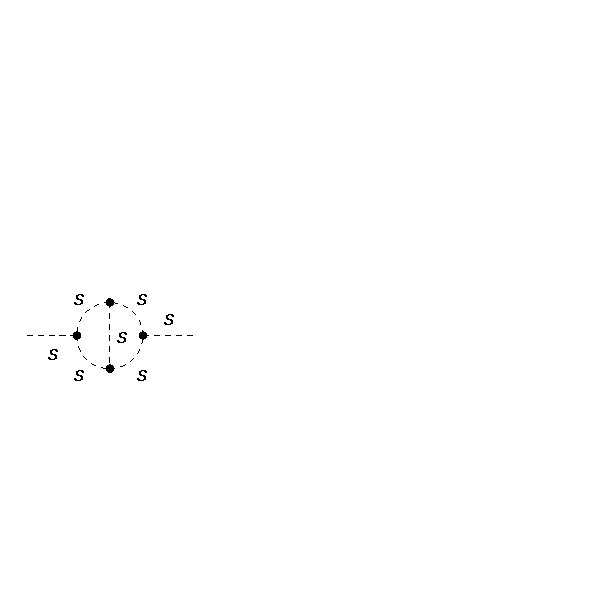
\includegraphics{2loop_4.pdf}
\end{center}
\begin{align}
\Pi_4 = \kappa^2 \frac{g^4}{2} \mathbf{TFI}(m^2,m^2,m^2,m^2,m^2)
\end{align}

Accounting for the negative sign and using the relationship $\mathbf{TFI}=\mathbf{M}$ we obtain the same result as the notes
\begin{align}
\Pi_4 = - \kappa^2 \frac{g^4}{2} \mathbf{M}(m^2,m^2,m^2,m^2,m^2)
\end{align}

\subsection*{Diagram 5}
\begin{center}
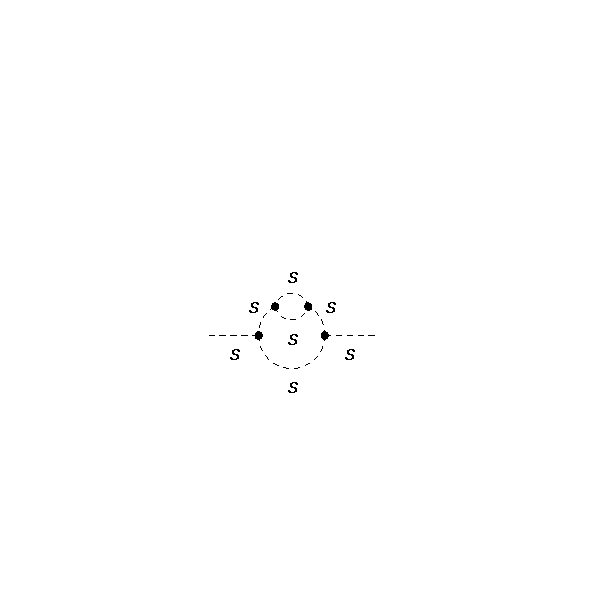
\includegraphics{2loop_5.pdf}
This diagram is given by TARCER to be after full reduction

\end{center}
\begin{align}
\begin{split}
\Pi_5 =& \kappa^2 \frac{g^4}{12 m^4} \left( \frac{3(3D-8)m^2(2m^2-p^2)}{p^2(4m^2-p^2)}\mathbf{TJI}(m^2,m^2,m^2)\right. \\
&+ \frac{4m^2(m^2-p^2)(9m^2-p^2)}{p^2(4m^2-p^2)}\mathbf{TJI}_2(m^2,m^2,m^2)\\
&+\frac{3(D-2)m^2(2m^2-p^2)}{p^2(4m^2-p^2)}\mathbf{TKI}(m^2,m^2,m^2)\\
&+\frac{m^2(D p^2+2(D-9)m^2)}{4m^2-p^2}\mathbf{TVI}(m^2,m^2,m^2,m^2)\\
&\left.+2(D-2)\mathbf{TAI}(m^2) \mathbf{TBI}(m^2,m^2) \right)
\end{split}
\end{align}
accounting for the negative sign and converting to TSIL notation we obtain

\begin{align}
\begin{split}
\Pi_5 =& - \kappa^2 \frac{g^4}{12 m^4} \left( \frac{3(3D-8)m^2(2m^2-p^2)}{p^2(4m^2-p^2)}\mathbf{S}(m^2,m^2,m^2)\right. \\
&-\frac{4m^2(m^2-p^2)(9m^2-p^2)}{p^2(4m^2-p^2)}\mathbf{T}(m^2,m^2,m^2)\\
&+\frac{3(D-2)m^2(2m^2-p^2)}{p^2(4m^2-p^2)}\mathbf{I}(m^2,m^2,m^2)\\
&-\frac{m^2(D p^2+2(D-9)m^2)}{4m^2-p^2}\mathbf{U}(m^2,m^2,m^2,m^2)\\
&\left.+2(D-2)\mathbf{A}(m^2) \mathbf{B}(m^2,m^2) \right)
\end{split}
\end{align}


\subsection*{Diagram 6}
\begin{center}
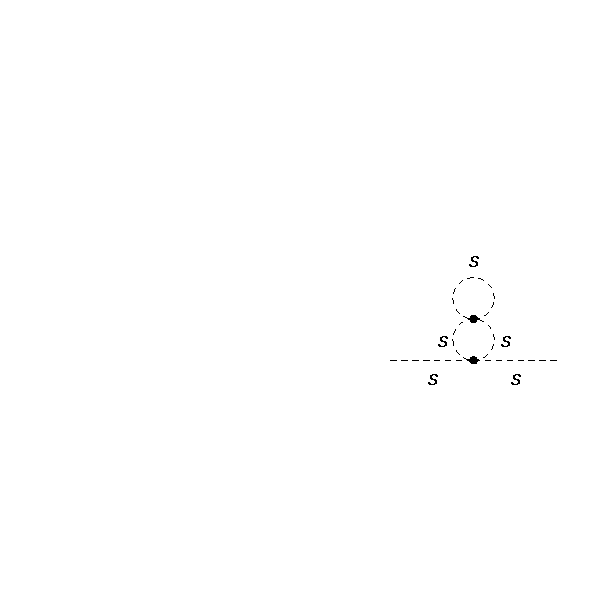
\includegraphics{2loop_6.pdf}
\end{center}
This diagram is given by TARCER to be
\begin{align}
\Pi_6 &= \kappa^2 \frac{\lambda^2(D-2)}{8}\frac{ \left({\tt{\mathbf{TAI}}} (m^2)\right)^2}{ m^2 }  
\end{align}
converting to TSIL notation and accounting for the negative sign we obtain
\begin{align}
\Pi_6 &= \kappa^2 \frac{\lambda^2(D-2)}{8}\frac{ \left({\tt{\mathbf{A}}} (m^2)\right)^2}{ m^2 }  
\end{align}

now we must set $D=4-r\epsilon$ and account for finite contributions which come from the divergent parts of the basis integrals.  I leave the factor of $r$ in for now.  The basis integrals can be expressed as a finite piece plus a divergent piece, so we have
\begin{align}
{\tt{\mathbf{TAI}}}(x) &= \frac{ix}{\epsilon} +  {\tt{TAI}}(x)
\end{align}
where we have converted \textcolor{blue}{(1.28)} of the TSIL manual into the TARCER definition using $\mathbf{A}= ia \tt{\mathbf{TAI}}$ and taking $a=1$ for small $\epsilon$ \footnote{I have tried keeping these additional $\epsilon$ terms in here coming from the $a$ factor, but I have found it leads to only more problems and additional terms which don't make sense to me.  Although I'm still a little uncertain, I have convinced myself taking $\epsilon \rightarrow 0$ for converting between these different normalisations is okay in this context.}.  So the amplitude becomes
\begin{align*}
\Pi_1 &= \frac{\lambda^2(2-r\epsilon)}{8 m^2 }       \left( {\tt{TAI}}(m^2) +\frac{im^2}{\epsilon}\right)^2  \\
&= \frac{\lambda^2}{4 m^2 }  {\tt{TAI}}(m^2) \left( \frac{ {\tt{TAI}}(m^2) } {m^2} - ir\right)
\end{align*}
where we ignore any divergent terms (assuming these will be cancelled by the counter-terms) and take the limit of $\epsilon\rightarrow 0$.
Finally we need to evaluate this in terms of TSIL integrals, which have a different normalization.  The relationship is $\mathbf{A}= ia \tt{\mathbf{TAI}}$ where $a = (4\pi\mu^2)^{2-D/2} \approx 1 +\frac{r\epsilon}{2}\log(4\pi\mu^2)+\mathcal{O}(\epsilon^2)$.  Since we have already removed the divergent parts and are dealing with finite integrals, I take $\epsilon =  0$ and we simply have $\mathbf{A}= i \tt{\mathbf{TAI}}$.  Therefore we end up with, after setting $r=2$ and taking account for the negative sign as with all other integrals,
\begin{align}
\Pi_1 & = \kappa^2  \frac{\lambda^2}{4 } A(m^2) \left( \frac{A(m^2)}{m^2} + 2 \right)
\end{align}




\subsection*{Diagram 7}
\begin{center}
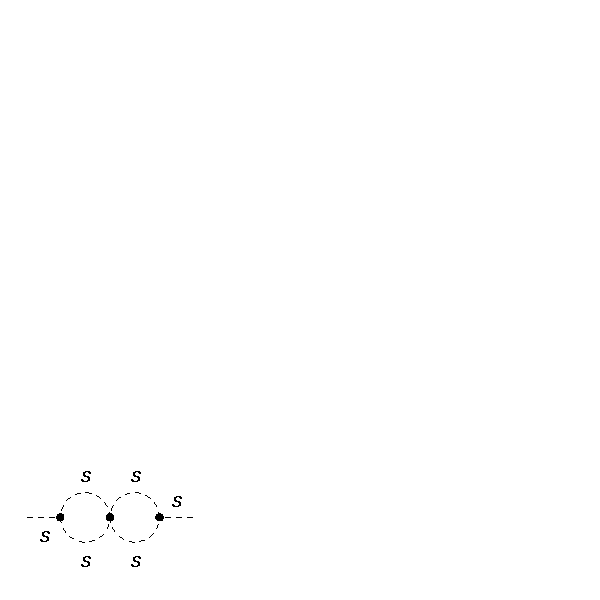
\includegraphics{2loop_7.pdf}
\end{center}
This diagram is given by TARCER to be
\begin{align}
\Pi_7 & =  \kappa^2 \frac{g^2 \lambda}{4 } \left(\mathbf{TBI}(m^2,m^2)\right)^2
\end{align}
accounting for negative sign and using $-i\mathbf{TBI} = \mathbf{B}$ we obtain
\begin{align}
\Pi_7 & = \kappa^2 \frac{g^2 \lambda}{4 } \left(\mathbf{B}(m^2,m^2)\right)^2
\end{align}


\subsection*{Diagram 8}
\begin{center}
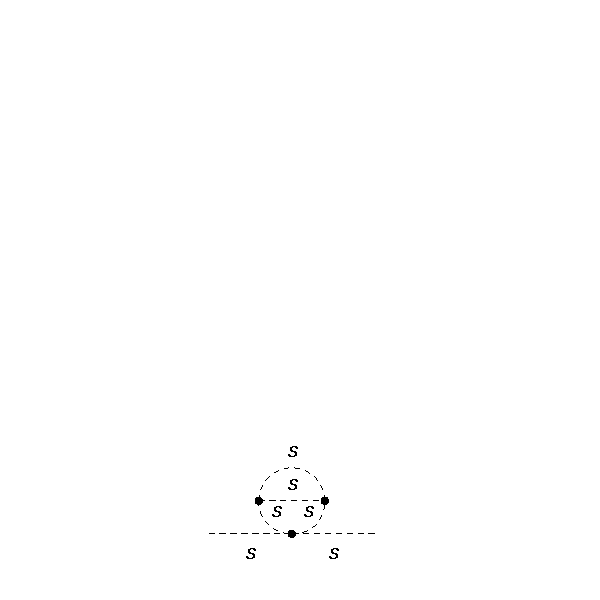
\includegraphics{2loop_8.pdf}
\end{center}
This diagram is given by TARCER to be
\begin{align}
\Pi_8 & = - \kappa^2\frac{g^2 \lambda}{12 m^2 } (D-3) \mathbf{TKI}(m^2,m^2,m^2)
\end{align}
converting to TSIL notation and accounting for the negative sign
\begin{align}
\Pi_8 & =  \kappa^2\frac{g^2 \lambda}{12 m^2 } (D-3) \mathbf{I}(m^2,m^2,m^2)
\end{align}
but we need another negative sign for the definition of K (apparently, check this)
\begin{align}
\Pi_8 & =  -\kappa^2\frac{g^2 \lambda}{12 m^2 } (D-3) \mathbf{I}(m^2,m^2,m^2)
\end{align}

\subsection*{Diagram 9}
\begin{center}
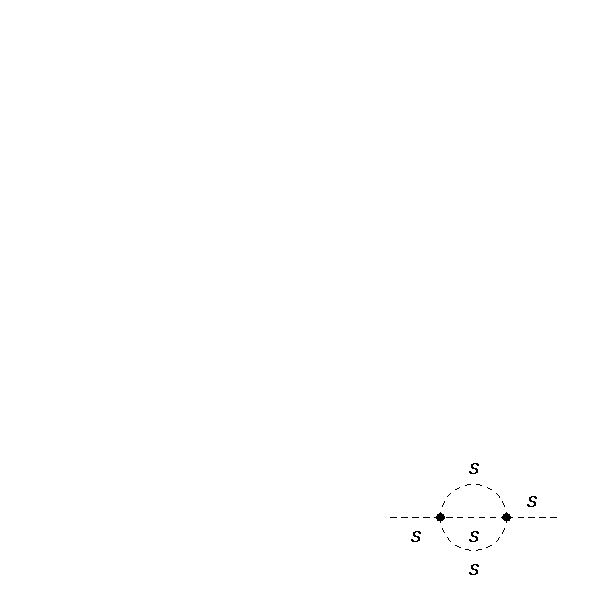
\includegraphics{2loop_9.pdf}
\end{center}
This diagram is given by TARCER to be

 \begin{align}
 \Pi_9 =\kappa^2 \frac{\lambda^2 {\tt{\mathbf{TJI}}}(m^2,m^2,m^2) }{6}
 \end{align}
 where ${\tt{\mathbf{TJI}}} = {\tt{\mathbf{TJI}}}\{1,1,1\}$ which is equivalent to the TSIL integral $S(x,y,z)$ for $a=1$, accounting for the negative sign we obtain
 \begin{align*}
 \Pi_9 & = -\kappa^2\frac{\lambda^2}{6}\textbf{S}(m^2,m^2,m^2)
 \end{align*}
 
 
 
 \section*{Counter-terms}
 
 
 The two-loop order counter-terms cancel divergences from the loop corrections and provide finite contributions to the total self energy.  In the MS bar scheme the counter-term couplings are of at least first order in $\mathcal{O}(1/\epsilon)$, so we can identify which counter-term diagrams will contribute finite contributions.
 
 
 
 
 \subsection*{Counter-diagram 1}
\begin{center}
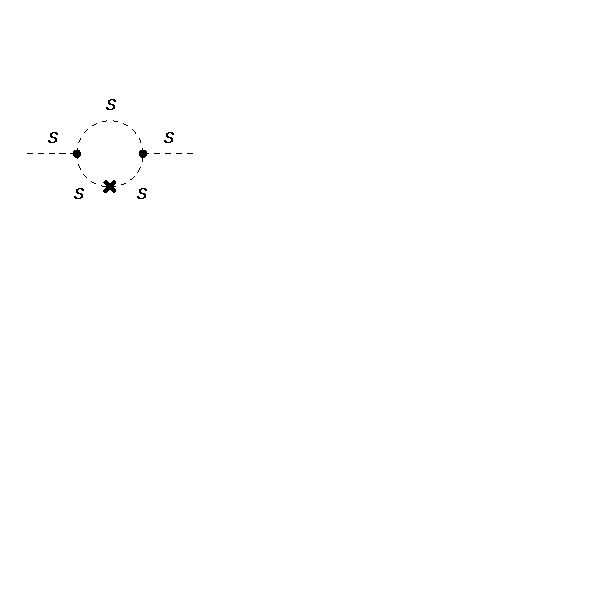
\includegraphics{2loop_1c.pdf}
\end{center}
 
 \begin{align}
 \Pi_1 = \kappa \frac{i  d_1 g^2}{ 2 m^2 (4m^2-p^2)} \left( (D-2){\tt{\mathbf{TAI}}}(m^2)-2(D-3){\tt{\mathbf{TBI}}}(m^2,m^2) \right)  
 \end{align}
 
 converting to TSIL notation, accounting for the negative sign and multiplying by $1/\epsilon$ we obtain
  \begin{align}
 \Pi_1 = \kappa \frac{ d_1 }{\epsilon}\frac{g^2}{ 2 m^2 (4m^2-p^2)} \left( (2-2\epsilon){\tt{\mathbf{A}}}(m^2)+2(1-2\epsilon){\tt{\mathbf{B}}}(m^2,m^2) \right)  
 \end{align}
 from which we obtain the finite contributions
\begin{align}
 \Pi_1 = \kappa d_1 \frac{g^2}{ 2 m^2 (4m^2-p^2)} \left( -2 A(m^2)+2A_{\epsilon}(m^2)-4m^2B(m^2,m^2)+2Bm^2_{\epsilon}(m^2,m^2)\right)
 \end{align}
 
  \subsection*{Counter-diagram 2}
 \begin{center}
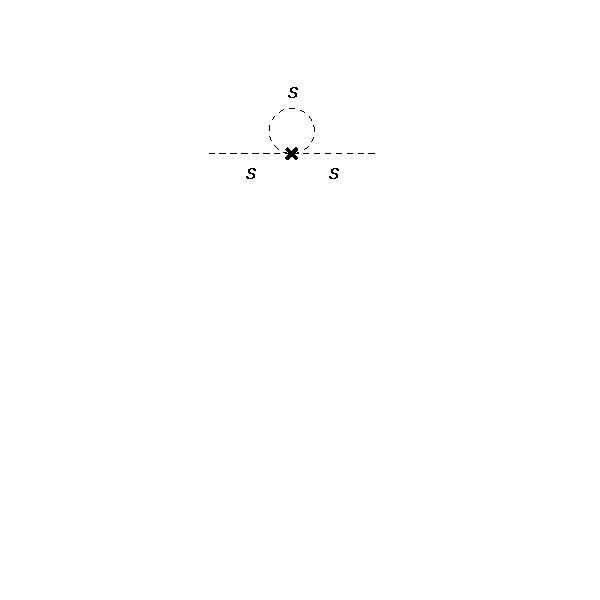
\includegraphics{2loop_2c.pdf}
\end{center}

 \begin{align}
 \Pi_2 = - \kappa i  \frac{d_{\lambda}}{2} {\tt{\mathbf{TAI}}}(m^2)
 \end{align}
 which after accounting for the negative sign and converting from TARCER to TSIL we obtain
  \begin{align}
 \Pi_2 = - \kappa \frac{d_{\lambda}}{2} \ {\tt{\mathbf{A}}}(m^2)
 \end{align}
 
   \subsection*{Counter-diagram 3 and 5}
 \begin{center}
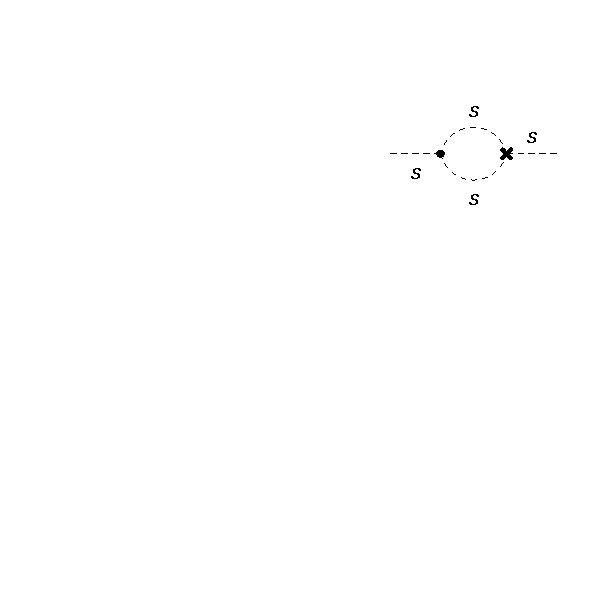
\includegraphics{2loop_3c.pdf} \ \ \ \ \ \ \ 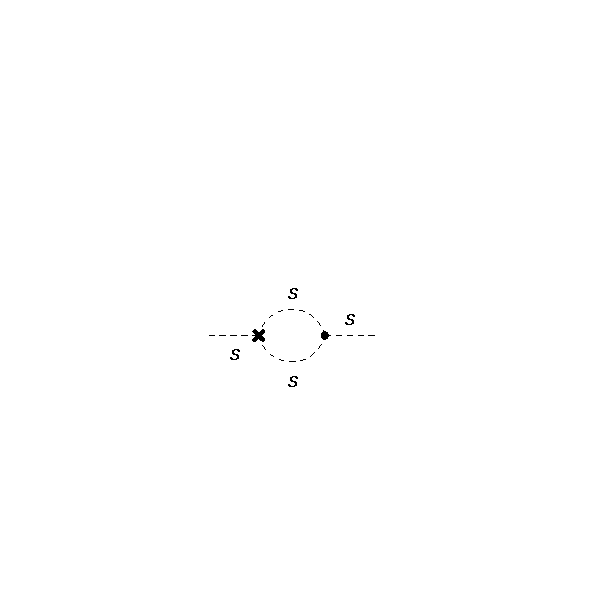
\includegraphics{2loop_5c.pdf}
\end{center}

 \begin{align}
 \Pi_{3,5} = - \kappa i \frac{g d_g}{2} {\tt{\mathbf{TBI}}}(m^2,m^2) 
 \end{align}
  
Combining these together and accounting for the negative sign we obtain
 \begin{align}
 \Pi_{3,5} = i \kappa g d_g {\tt{\mathbf{TBI}}}(m^2,m^2) 
 \end{align}
converting to TSIL notation and inserting the counter-term coupling (each introduces a negative sign)
\begin{align}
 \Pi_{3,5} = \kappa^2 g \frac{c_{1,1}^g}{\epsilon} {\tt{\mathbf{B}}}(m^2,m^2) 
 \end{align}

 
\subsection*{Counter-diagram 4}
\begin{center}
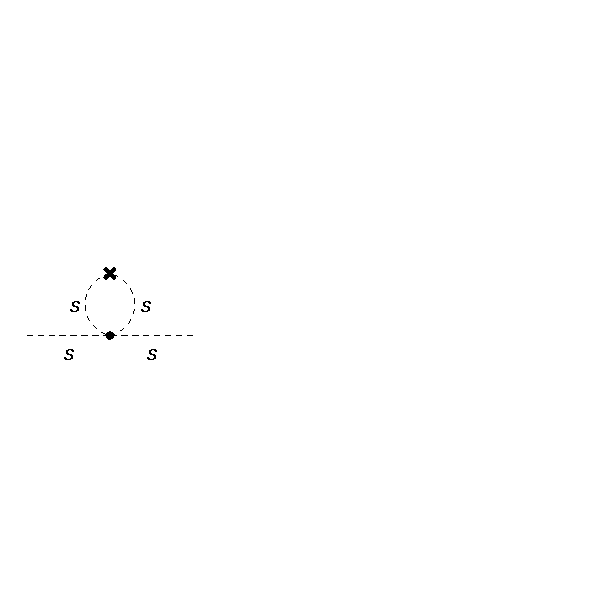
\includegraphics{2loop_4c.pdf}
\end{center}

 \begin{align}
 \Pi_4 =  \kappa \frac{-i \lambda d_1 (D-2)}{ 4 m^2} {\tt{\mathbf{TAI}}}(m^2) 
 \end{align}
 
 accounting for the negative sign and changing notation we obtain
 \begin{align}
 \Pi_4 =  \kappa \frac{ \lambda d_1 (D-2)}{ 4 m^2} {\tt{\mathbf{A}}}(m^2) 
 \end{align}
 
 


 \section*{Comments}
 
 In Stephen's working the $A_{\epsilon}(x')$ terms cancel between the diagrams and the counter-term diagrams.  However,
 
 \begin{align*}
 A_{\epsilon}(x') = \frac{A_{\epsilon}(x)}{x}-\frac{A(x)}{x}
 \end{align*}
 
 so there is actually a $A(x)$ term here that is cancelling out between the normal diagrams and the finite contribution from the counter-terms, but it's kind of hidden.  In our approach, we do not invoke this derivative at all (and don't carry around non-expanded things like  $A_{\epsilon}(x')$ ) , and thus our diagram (diagram 5) explicitly contains this $A(x)$ term, so it appears wrong until we actually consider the counter-term.  In Stephen's approach we could actually just ignore the  $A_{\epsilon}(x')$  term from the beginning knowing it will cancel.  All this only becomes apparent when we expand out  $A_{\epsilon}(x')$ and look at the counter-term and normal diagrams separately.
 
 



\section{The electroweak triplet model}
\subsection{Introduction}

The extension of the standard model by an electroweak multiplet is a common procedure to produce a dark matter candidate.  At the lowest order in perturbation theory all components of the multiplet have the same mass, which would result in charged dark matter, contrary to what is observed.  However when one goes to the next order in perturbation theory by computing the radiatively corrected mass, then the charged components obtain a slightly larger mass correction that the neutral component, resulting in a sufficient mass splitting to render the charged components to have a lifetime much shorter than the age of the universe.  The exact value of this mass splitting at the two-loop level is of interest.  We will work with the most simple multiplet, a triplet, to determine the value of this mass splitting at the two-loop order in perturbation theory.



For these calculations we use a triplet electroweak extension to simplify the number of interactions required to compute the mass splitting between the neutral and charged component.  The Lagrangian is then
\begin{align}
\begin{split}
\mathcal{L}=&\mathcal{L}_{\text{SM}}+\frac{1}{2}\overline{\mychi^0}(i\slashed{\partial}-M)\mychi^0+\frac{1}{2}\overline{\mychi^+}(i\slashed{\partial}-M)\mychi^{+}\\
&+g\left(\overline{\mychi^+}\gamma_{\mu}\mychi^+\right)\left(s_wA_{\mu}+c_wZ_{\mu}\right)\\
&+g\left(\overline{\mychi^+}\gamma_{\mu}\mychi^0 \right)W_{\mu}^++\text{h.c.}
\end{split}
\end{align}

The momentum dependent contribution to the triplet mass, the self energy, is given by calculating the 1PI loop process.  For the $
\chi^0$ at one loop level this involves a loop with a W boson and $\chi^{\pm}$ particle, for $\chi^{\pm}$ we also have loops involving $
\chi^{\pm\pm}$, $W^{\pm}$ and the $A$ and $Z$ bosons.  The propagators we will use are (in the Feynman gauge)

\begin{align}
i\Pi^{W^{\pm}}_{\mu\nu}&=-i\frac{-g_{\mu\nu}}{k^2-m_{\text{w}}^2}\\
i\Pi^{\chi^{0}}_{\mu\nu}&=i\Pi^{\chi^{\pm}}_{\mu\nu}=i\Pi^{\chi^{\pm\pm}}_{\mu\nu}=-i\frac{\slashed{k}-m}{k^2-m^2}\\
i\Pi^{A}_{\mu\nu}&=-i\frac{-g_{\mu\nu}}{k^2-m_A^2}\\
i\Pi^{Z^{\pm}}_{\mu\nu}&=-i\frac{g_{\mu\nu}}{k^2-m_z^2}\\
\end{align}


where $m$ is taken to the be the degenerate (tree-level) triplet mass.

\section{One-loop self energy}
\begin{figure}[h!]
\center
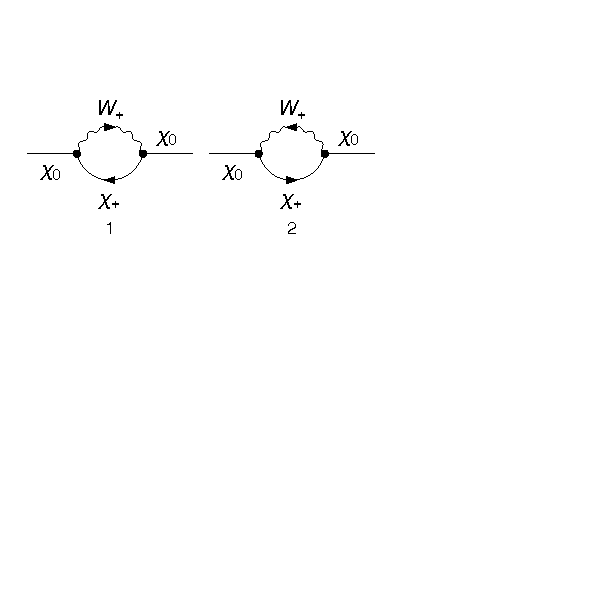
\includegraphics[width=0.6\textwidth]{1loop.pdf}\\
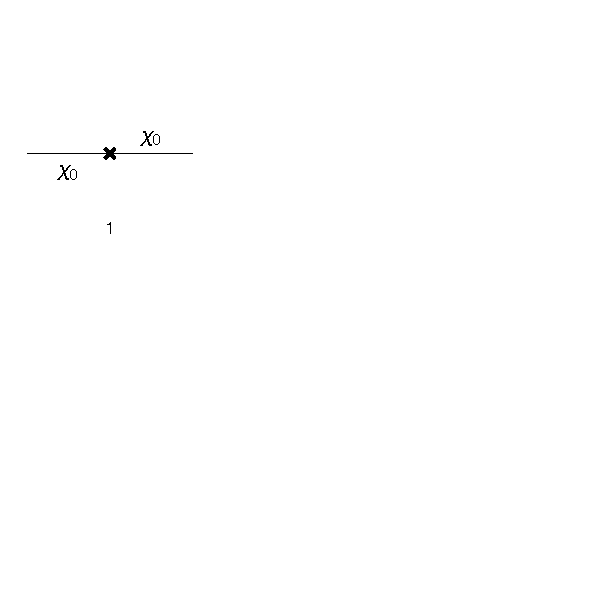
\includegraphics[width=0.3\textwidth]{1loop_1c.pdf}\\
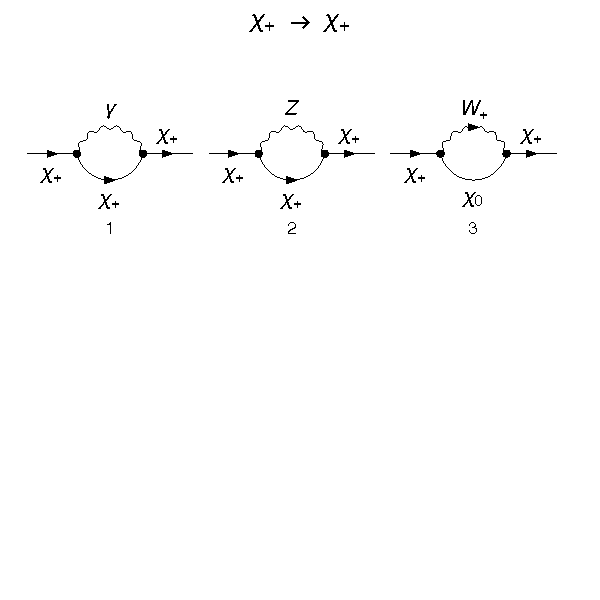
\includegraphics[width=0.8\textwidth]{diagrams_F[1]_1.pdf}
\caption{The one-loop order loop (\textit{top}) and counter-term (\textit{bottom}) corrections to the scalar propagator.}\label{fig:1loop_chi}
\end{figure}

The processes which contribute the one-loop self energy are given in Figure \ref{fig:1loop_chi} for both the charged and neutral components.  We will present a detailed calculation of the one-loop self energy for the purposes of illustration.


\subsubsection{Neutral component}

The neutral component only has one possible radiative correction, due to the processes $\chi_0\rightarrow W^{\pm} + \chi^{\mp}$, so the loop integral we need to evaluate is

\begin{align}
i\Sigma_{\cn}(\slashed{p})&= 2 (-\sqrt{3}gi)^2 \int \frac{\d^4k}{(2\pi)^4} \gamma^{\mu}\frac{(\slashed{p}-\slashed{k}+m)\gamma^{\nu}\left(-g_{\mu\nu}\right)}{((p-k)^2-m^2)(k^2-m_{\text{w}}^2)}\label{eqn:cn_loop}
\end{align}
where we have included a factor of two since this process can occur via either $\chi_0\rightarrow W^+ + \chi^-$ or $\chi_0\rightarrow W^- + \chi^+$.  Evaluating this integral using FeynCalc gives, with $\sp=m$
\begin{align}
\Sigma_{\cn}(m)= \frac{12g^2}{(4\pi)^2} m \left(\frac{1}{2}+2B_0(m^2,m^2,m_{\text{w}}^2)+B_1(m^2,m^2,m_2^2)\right)
\end{align}



\subsubsection{Charged component}

The charged component has radiative corrections from four processes, these are
\begin{align*}
\chi^{-}&\rightarrow \overline{\chi^{-}}+A\\
\chi^{-}&\rightarrow \overline{\chi^{-}}+Z\\
\chi^{-}&\rightarrow \overline{\chi^{0}}+W^-\\
\chi^{-}&\rightarrow \overline{\chi^{--}}+W^+
\end{align*}
the loop integrals required for each of these processes are similar to, or simpler, than that for the neutral component.  These are

\begin{align}
\begin{split}
i\Sigma_{\cm}(\slashed{p})=&\left((-\sqrt{3}gi)^2+(-\sqrt{2}gi)^2\right) \int \frac{\d^4k}{(2\pi)^4} \gamma^{\mu}\frac{(\slashed{p}-\slashed{k}+m)\gamma^{\nu}\left(-g_{\mu\nu}\right)}{((p-k)^2-m^2)(k^2-m_{\text{w}}^2)}\\
&+(-is_w)^2 \int \frac{\d^4k}{(2\pi)^4} \gamma^{\mu}\frac{(\slashed{p}-\slashed{k}+m)\gamma^{\nu}\left(-g_{\mu\nu}\right)}{((p-k)^2-m^2)(k^2)}\\
&+(-ic_w)^2 \int \frac{\d^4k}{(2\pi)^4} \gamma^{\mu}\frac{(\slashed{p}-\slashed{k}+m)\gamma^{\nu}\left(-g_{\mu\nu}\right)}{((p-k)^2-m^2)(k^2-m_{\text{z}}^2)}
\end{split}
\end{align}
where $s_w=\sin(\theta_w)$ and $c_w=\cos(\theta_w)$ are the sine and cosine of the Weinberg angle respectively.  Evaluating this integral in FeynCalc, with $D=4$ and $\sp=m$ gives
\begin{align}
\begin{split}
\Sigma_{\cm}(m)=& \frac{2g^2}{(4\pi)^2} m \left[  -5(2B_0(m^2,m^2,m_{\text{w}}^2)+B_1(m^2,m^2,m_{\text{w}}^2)) \right.\\ & -c_w^2 (2B_0(m^2,m^2,m_{\text{z}}^2)+B_1(m^2,m^2,m_{\text{z}}^2)) \\&\left.-s_w^2(2B_0(m^2,m^2,0)+B_1(m^2,m^2,0))\right]\label{eqn:charged_SE}
\end{split}
\end{align}




\subsubsection{Details of integration}

We will calculate the neutral component self energy by hand to confirm that the FeynCalc output is correct.  The loop integral is expressed as
\begin{align}
i\Sigma_{\cn}(\slashed{p})&= 2(-\sqrt{3}gi)^2 \int \frac{\d^4k}{(2\pi)^4} \frac{N}{((p+k)^2-m^2)(k^2-m_{\text{w}}^2)}
\end{align}
where we simplify $N$ by
\begin{align*}
N&=-\gm(\sk+\sp+m)\gn g_{\mu\nu}\\
&=-\gm(\sk+\sp+m)\gamma_{\mu}\\
&=2(\sk+\sp)-4m
\end{align*}
%\begin{align}
%M&=\gm(\sk+\sp+m)\gn(\km\kn)\\
%&=m\sk\sk+\gm(p_{\rho}+\kp)\gp\km\sk\\
%&=m\sk\sk+(p_{\rho}+\kp)\gm\gp\km\sk\\
%&=m\sk\sk+(p_{\rho}+\kp)(-\gp\gm+2g^{\rho\mu})\km\sk\\
%&=m\sk\sk-(\sk+\sp)\sk\sk+2(k^{\mu}p_{\mu}+k^{\mu}\km)I_4\sk\\
%&=m\sk\sk-\sk\sk\sk-\sp\sk\sk-\sp\sk\sk+\sk\sp\sk+\sp\sk\sk+2\sk\sk\sk\\
%&=m\sk\sk+\sk\sp\sk+\sk\sk\sk=\sk(m+\sp+\sk)\sk
%\end{align}
using the identities
\begin{align}
\begin{split}
\gamma_{\mu}\slashed{a}\gm&=-2\slashed{a}\\
\gm\gamma_{\mu}&=4I_4
\end{split}
\end{align}
where $I_4$ is the identity matrix in 4 dimensions.
%(I have realised now I should include the factor $I_4$ throughout these calculations, however I am confused about this a bit.  Any term that has a $\slashed{p}$ for example, is actually a ``matrix", the terms where all momentum has been contracted, like the $-4m$ in $N$, I should really be carrying around this identity.  I also don't know if I'm meant to take a trace at the end of all this, like we do for amplitudes when there are free spinor indices, yet in this case everything is contracted.  I am also confused about setting $\slashed{p}=m$, as I have seen in my text book, this should really be $\slashed{p}=mI_4$, right?).

Now we use the Feynman parameter integral
\begin{align}
\frac{1}{AB}=\int_0^1 \frac{\d x}{[A+(B-A)x]^2}
\end{align}
to simplify the denominator
\begin{align*}
 \frac{1}{((p-k)^2-m^2)(k^2-m_{\text{w}}^2)}&=\int_0^1\frac{\d x}{[k^2-m_{\text{w}}^2+(p^2-2kp+k^2-(k^2-m_{\text{w}}^2))x]^2}\\
&=\int_0^1\frac{\d x}{[ k^2-2kpx+p^2x+x(m_{\text{w}}^2-m^2)-m_{\text{w}}^2]^2}\\
&=\int_0^1\frac{\d x}{[ (k-px)^2+x(1-x)p^2+x(m_{\text{w}}^2-m^2)-m_{\text{w}}^2]^2}\\
&=\int_0^1\frac{\d x}{[ k'-\Delta]^2}
\end{align*}
where $k'=k-px$ and $\Delta=-x(1-x)p^2-x(m_{\text{w}}^2-m^2)+m_{\text{w}}^2$.


%So the loop integral is now
%\begin{align}
%i\Sigma_{\cn}(\slashed{p})&= (-3gi)^2 \int \frac{\d^4k}{(2\pi)^4} \frac{2(\sk+\sp)-4m+\sk(m+\sp+\sk)\sk/m_{\text{w}}^2}{((p+k)^2-m^2)(k^2-m_{\text{w}}^2)}
%\end{align}
%{\textbf{ This is the form of the integral I entered into FeynCalc.}}

We now translate the integration measure $\int \d^4k\rightarrow\int \d^4k'$ (and henceforth omitting the prime on $k'$) to obtain (after substituting $k\rightarrow k+px$ in the numerator)
\begin{align}
i\Sigma_{\cn}(\slashed{p})&= 2(-\sqrt{3}gi)^2 \int \frac{\d^4k}{(2\pi)^4}\int_0^1 \d x \frac{2(\sp(1-x)-\sk )-4m}{[ k^2-\Delta]^2}
\end{align}
after shifting the integration measure.

%We must now simplify $N$ and $M$ again to be able to carry out the integration over $k$ more easily (it may appear that we could have left $M$ in it's original form, and simplified only once after the momentum translation.  However, both methods require the same manipulations to be done at some point, so we choose to put it in a tidy form first, particularly for use in FeynCalc).
%
%\begin{align*}
%M=&(\sk-x\sp)(m+\sp+(\sk-x\sp))(\sk-x\sp)\\
%=&(\sk\sp+\sk\sk-x\sp\sp-2x\kmpm+x^2\sp\sp)(\sk-x\sp)+m(\sk-x\sp)(\sk-x\sp)\\
%=&\sk\sp\sk-2x\kmpm\sk-x\sk\sk\sp+x^2\sp\sp\sp-x^2\sp\sp\sp+m(k^2+x^2p^2)\\
%&+\sk\sk\sk-x\sp\sp\sk-x\sk\sp\sp+2x^2\kmpm\sp+x^2\sp\sp\sk-2m\kmpm\\
%\end{align*}


since the denominator of the loop integral is symmetric with respect to $k$ we can discard all terms here of odd order in $k$, thus
\begin{align}
i\Sigma_{\cn}(\slashed{p})&= 2(-\sqrt{3}gi)^2 \int \frac{\d^4k}{(2\pi)^4}\int_0^1 \d x \frac{2(\sp(1-x))-4m}{[ k^2-\Delta]^2}
\end{align}



%\begin{align}
%M=&-\sp(1+x)k^2+2p^{\mu}\gn(1-x)\km\kn+\sp p^2(x^2-x^3)+m(k^2+x^2p^2)
%\end{align}

%Likewise for $N$ we have
%\begin{align}
%N&=2((\sk-x\sp)+\sp)-4m=2\sp(1-x)-4m
%\end{align}
%
%
%Therefore we have the integral
%
%\begin{align}
%i\Sigma_{\cn}(\slashed{p})= &-3g^2\int \frac{\d^4k}{(2\pi)^4} \int_0^1 \d x \left[  \frac{ 2\sp(1-x)-4m}{[ k^2-\Delta]^2}\right.+\\
%& \left.\frac{ -\sp(1+x)k^2+2p^{\mu}\gn(1-x)\km\kn+\sp p^2(x^2-x^3)+m(k^2+x^2p^2)}{m_{\text{w}}^2[ k^2-\Delta]^2}\right]
%\end{align}
%we will deal with each power of $k$ separately, so we express the integral as
%
%\begin{align}
%i\Sigma_{\cn}(\slashed{p})_{k^2}=&-3g^2\int \frac{\d^4k}{(2\pi)^4} \int_0^1 \d x \frac{1}{m_{\text{w}}^2} (-\sp(1+x)+m) \frac{k^2}{[ k^2-\Delta]^2}\\
%i\Sigma_{\cn}(\slashed{p})_{\km\kn}= &-3g^2\int \frac{\d^4k}{(2\pi)^4} \int_0^1 \d x \frac{1}{m_{\text{w}}^2}(2p^{\mu}\gamma^{\mu}(1-x)) \frac{\km\kn}{[ k^2-\Delta]^2}  \\
%i\Sigma_{\cn}(\slashed{p})_0=&-3g^2\int \frac{\d^4k}{(2\pi)^4} \int_0^1 \d x\left( 2\sp(1-x)-4m+\frac{\sp p^2(x^2-x^3)+mx^2p^2}{m_{\text{w}}^2}\right)  \frac{1}{[ k^2-\Delta]^2}
%\end{align}

%For each of these integrals we use dimensional regularisation, since in each case the factor immediately after the integrand is independent of $k$ we can ignore this for now and deal with the $k$ dependent terms.

Now we apply dimensional regularisation, letting $d=4-\epsilon$, such that in the limit of small $\epsilon$ we have
%\begin{align*}
%\int \frac{\d^4k}{(2\pi)^4}  \frac{\km\kn}{[ k^2-\Delta]^2} &\rightarrow  \mu^{\epsilon}\int \frac{\d^dk}{(2\pi)^d}  \frac{\km\kn}{[ k^2-\Delta]^2}\\
%&= \frac{-ig_{\mu\nu}}{2}\frac{1}{\Delta^{1-\frac{d}{2}}}\Gamma\left(\frac{2-d}{2}\right)\frac{1}{(4\pi)^{\frac{d}{2}}}\\
%&= \frac{-ig_{\mu\nu}}{2(4\pi)^2}\frac{\Delta}{\Delta^{\epsilon/2}}\Gamma\left(\frac{\epsilon}{2}-1\right) (4\pi)^{\epsilon/2}\\
%&= \frac{-ig_{\mu\nu}}{2(4\pi)^2}\frac{\Delta}{\Delta^{\epsilon/2}}\Gamma\left(\frac{\epsilon}{2}\right) \left(\frac{\epsilon}{2}-1\right)^{-1}(4\pi)^{\epsilon/2}\\
%&\approx \frac{ig_{\mu\nu}\Delta}{2(4\pi)^2} \left( 1-\he\log\Delta\right)\left(\frac{2}{\epsilon}-\gamma\right)\left(1+\he\right)\left(1+\he\log 4\pi\right)\left(1+\he\log\mu^2\right)\\
%&=\frac{ig_{\mu\nu}\Delta}{2(4\pi)^2} \left(\frac{2}{\epsilon}+1-\gamma+\log\frac{4\pi\mu^2}{\Delta}\right)+\mathcal{O}(\epsilon)
%\end{align*}
%where we have used the fact that $n\Gamma(n)=\Gamma(n+1)$ and thus
%$$
%\left(\frac{\epsilon}{2}-1\right)\Gamma\left(\frac{\epsilon}{2}-1\right)=\Gamma\left(\frac{\epsilon}{2}\right).
%$$
%and 
%$$
%\left(\frac{\epsilon}{2}-1\right)^{-1}\approx -1-\frac{\epsilon}{2}
%$$
%The calculation is similar for $k^2$
%\begin{align}
%\int \frac{\d^4k}{(2\pi)^4}  \frac{k^2}{[ k^2-\Delta]^2} &\rightarrow  \mu^{\epsilon}\int \frac{\d^dk}{(2\pi)^d}  \frac{\km\kn}{[ k^2-\Delta]^2}\\
%&\approx\frac{i(4-\epsilon)\Delta}{2(4\pi)^2} \left(\frac{2}{\epsilon}+1-\gamma+\log\frac{4\pi\mu^2}{\Delta}\right)+\mathcal{O}(\epsilon)\\
%&=\frac{2i\Delta}{(4\pi)^2} \left(\frac{2}{\epsilon}+\frac{1}{2}-\gamma+\log\frac{4\pi\mu^2}{\Delta}\right)+\mathcal{O}(\epsilon)
%\end{align}
%and in the $k^0$ case the result is simpler to obtain, and we find




\begin{align*}
\int \frac{\d^4k}{(2\pi)^4}{[ k^2-\Delta]^2} &\rightarrow  \mu^{\epsilon}\int \frac{\d^dk}{(2\pi)^d}  \frac{1}{[ k^2-\Delta]^2}\\
&= \mu^{\epsilon}\frac{i}{(4\pi)^{\frac{d}{2}}} \frac{1}{\Delta^{2-\frac{d}{2}}} \Gamma\left(\frac{4-d}{2}\right) \\
&= \mu^{\epsilon}\frac{-i}{(4\pi)^2}\frac{1}{\Delta^{\epsilon/2}}\Gamma\left(\frac{\epsilon}{2}\right) (4\pi)^{\epsilon/2}\\
&\approx \frac{i}{(4\pi)^2} \left( 1-\he\log\Delta\right)\left(\frac{2}{\epsilon}-\gamma\right)\left(1+\he\log 4\pi\right)\left(1+\he\log\mu^2\right)\\
&=\frac{i}{(4\pi)^2} \left(\frac{2}{\epsilon}-\gamma+\log\frac{4\pi\mu^2}{\Delta}\right)+\mathcal{O}(\epsilon)
\end{align*}

We are now ready to calculate the integral for $i\Sigma_{\cn}(\slashed{p})$.

\begin{align}
i\Sigma_{\cn}(\slashed{p})&= 2(-\sqrt{3}gi)^2 \frac{i}{(4\pi)^2}  \int_0^1 \d x \left(2(\sp(1-x))-4m\right) \left(\frac{2}{\epsilon}+\log\frac{\hat{\mu}^2}{\Delta}\right)
\end{align}
where $\hat{\mu}^2=4\pi\mu^2e^{-\gamma}$.


%Starting with $i\Sigma_{\cn}(\slashed{p})_{k^2}$ we find
%
%\begin{align}
%\Sigma_{\cn}(\slashed{p})_{k^2}=\int_0^1\!\d x\ \frac{-3g^2}{(4\pi)^2m_{\text{w}}^2}2\left(-\sp(1+x)+m\right)\Delta\left(\frac{1}{2}+\log\frac{\hat{\mu}}{\Delta}\right)
%\end{align}
%where $\hat{\mu}=\mu^2e^{-\gamma}$ and we will henceforth neglect the divergent $2/\epsilon$ term, as we are interested in evaluating the finite part of the loop integral for use in the self energy.  Similarly,
%\begin{align}
%\Sigma_{\cn}(\slashed{p})_{\km\kn}&=\int_0^1\!\d x\ \frac{-3g^2}{(4\pi)^2m_{\text{w}}^2}\left(\sp(1-x)\right)\Delta\left(1+\log\frac{\hat{\mu}}{\Delta}\right)\\
%\Sigma_{\cn}(\slashed{p})_{0}&=\int_0^1\!\d x\ \frac{-3g^2}{(4\pi)^2}\left(   2\sp(1-x)-4m+\frac{\sp p^2(x^2-x^3)+mx^2p^2}{m_{\text{w}}^2}   \right)\log\frac{\hat{\mu}}{\Delta}
%\end{align}


%To simplify these integrals further we can take $p=\sp=m$, as is required when evaluating the self energy.  Then, we find the integrals
%
%\begin{align*}
%\Sigma_{\cn}(\slashed{p})=&\frac{-3g^2}{(4\pi)^2}\int_0^1\!\d x\ m\left[   -1+3x(-2+x) +\frac{m^3}{m_w^2}(x^2(3-4x)) \right]\\
%&+m\left[ (2x-1)(x-1)  +\frac{m^3}{m_{\text{w}}^2}\left(x^2(2x-1)\right)  \right]\left(\log\frac{\hat{\mu}}{\Delta}\right)\\
%\end{align*}

The Passarino-Veltman functions we have are (from arXiv:1212.5989)
\begin{align}
B_0(p^2,m_1^2,m_2^2)&=\int_0^1\!\d x \ \log\frac{\hat{\mu}}{\Delta}\\
B_1(p^2,m_1^2,m_2^2)&=-\int_0^1\!\d x \ x\log\frac{\hat{\mu}}{\Delta}
%B_{21}(p^2,m_1^2,m_2^2)&=\int_0^1\!\d x \ x^2\log\frac{\hat{\mu}}{\Delta}
\end{align}
where we have omitted the divergent part, if we assume MS occurs through the appropriate counter-terms then we need not work through this part here.  So, ignoring the divergent part in our integral as well we obtain the result
\begin{align}
i\Sigma_{\cn}(\slashed{p})&= 2(-\sqrt{3}gi)^2 \frac{i}{(4\pi)^2}  \left(2\sp\left( B_0(p^2,m_{\text{w}}^2,m^2)+B_1(p^2,m_{\text{w}}^2,m^2)\right)-4mB_0(p^2,m_{\text{w}}^2,m^2)\right)
\end{align}
such that if we let $\sp=m$
\begin{align}
\Sigma_{\cn}(m)&= \frac{-12mg^2}{(4\pi)^2}   \left( -B_0(m^2,m_{\text{w}}^2,m^2)+B_1(m^2,m_{\text{w}}^2,m^2)\right).
\end{align}
To bring it into the same form as given by FeynCalc and SARAH use the identity $B_1(p^2,m_1^2,m_2^2)=-B_1(p^2,m_2^2,m_1^2)-B_0(p^2,m_2^2,m_1^2)$ such that
\begin{align}
\Sigma_{\cn}(m)&= \frac{12mg^2}{(4\pi)^2}   \left( 2B_0(m^2,m^2,m_{\text{w}}^2)+B_1(m^2,m^2,m_{\text{w}}^2)\right)
\end{align}


\section{1-loop boson self energies}

To verify the method and FeynArts model we cross-check the boson self energies with that presented by Ibe et al.


The full 2-point propagator for the gauge bosons (in the Feynman gauge) is $(-ig_{\mu\nu})/[p^2 - \hat{m}_V^2 + \Pi(p^2)]$, where $\Pi(p^2)$ is the 1PI amplitude.



In this section we give the details of the one-loop contributions to this amplitude
,$\Pi(p^2)$, from all particles in our simplified EW triplet model.  These contributions are given by
{\small
\begin{eqnarray}
\Pi_{V_1 V_2}
= \Pi_{V_1 V_2}^{(V, h)}
+ \Pi_{V_1 V_2}^{(\tilde{\chi})}
+ p^2 \delta_{Z_{V_1 V_2}}
+ \delta_{m^2_{V_1 V_2}}\ ,
\end{eqnarray}
}where $V_1 V_2 =$ $\gamma \gamma$, $\gamma Z$, $ZZ$, and $WW$. The first term in the right-hand side is the contributions from the gauge-Higgs sector of the SM and the second term is from the electroweak triplet. 
The third and fourth terms are the one-loop counter-terms which we determine in the following section.


The following is a direct quote from BMPZ, please reword.
 \textcolor{red}{
The self-energies of the gauge-bosons can be separated into transverse
and longitudinal pieces, e.g.
%
\begin{equation}
\Pi^{\mu\nu}_{ZZ}(p^2) \ =\ \Pi_{ZZ}^T(p^2)\biggl[g^{\mu\nu}
-{p^{\mu}p^{\nu}\over p^2}\biggr] \ +\ \Pi_{ZZ}^L(p^2)\,
{p^{\mu}p^{\nu}\over p^2}\ .
\end{equation}
%
The physical gauge-boson masses are the poles of the corresponding
propagators, which involve only the transverse part of the gauge-boson
self-energy,
%
\begin{eqnarray}
&& M_Z^2 \ =\ \hat M_Z^2(Q) \ -\ {\cal
R}e\,\Pi^T_{ZZ}(M_Z^2)~,\label{mz}\\ && M_W^2 \ =\ \hat M_W^2(Q) \ -
\ {\cal R}e\,\Pi^T_{WW}(M_W^2)~.
\end{eqnarray}
%
Here $\hat M_Z(Q)$ and $\hat M_W(Q)$ denote the
\mbox{\footnotesize$\overline{\rm DR}~$} running masses which are
related to the \mbox{\footnotesize$\overline{\rm DR}~$} gauge
couplings and vev's, as in Eq.~(\ref{mwmz}). The gauge-boson
self-energies are evaluated at the renormalization scale $Q$.
}

\subsection{Photon self energy}

Consider the contributions to the photon self energy from Higgs and boson sector. 

\begin{figure}[h!]
\center
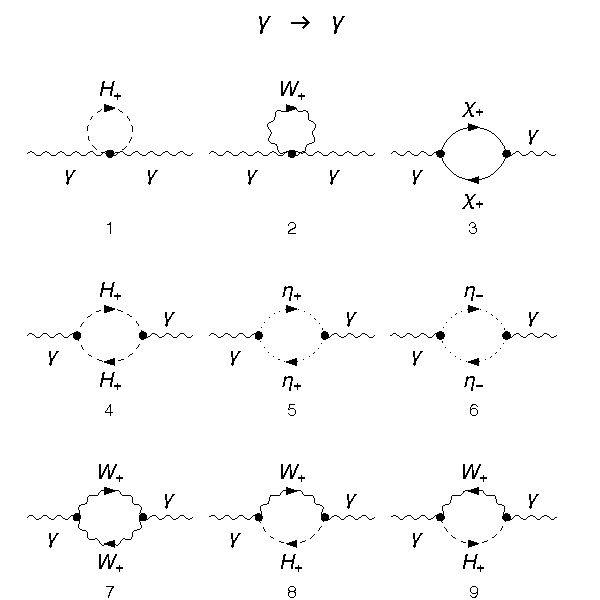
\includegraphics[width=0.6\textwidth]{diagrams_V[1]_1.pdf}
\caption{The one-loop corrections to the photon propagator.}\label{fig:gammagamma}
\end{figure}

From Ibe et al. we have
\begin{align}
\Pi_{\gamma \gamma}^{(V, h)}(p^2) =
-\frac{3 \hat{e}^2}{4\pi^2}
\left[ \tilde{B}_{22}(p^2, \hat{m}_W^2, \hat{m}_W^2) + \frac{p^2}{18} \right]
-\frac{\hat{e}^2 p^2}{4\pi^2} B_0(p^2, \hat{m}_W^2, \hat{m}_W^2)
\end{align}
where this includes all contributions from the 9 diagrams in Figure \ref{fig:gammagamma}.  We use the following relationships to compare the form given here with that produced from FeynCalc
\begin{align}
s_w^2&=\frac{g_1^2}{g_1^2+g_2^2}\\
c_w^2&=\frac{g_2^2}{g_1^2+g_2^2}\\
\alpha&=\frac{g_1^2g_2^2}{g_1^2+g_2^2}\\
v&=\frac{2m_w}{g_2}\\
\alpha&=e^2
\end{align}
We find the self energy contribution from FeynCalc in a fully reduced scheme is
\begin{align}
\Pi_{\gamma \gamma}^{(V, h)}(p^2) = \frac{\alpha}{32\pi^2} \left( \left(4m_W^2-6(2m_W^2+p^2)\right)B_0(m_W^2,m_W^2)+8 A_0(m_W^2)-8m_W^2\right)
\end{align}


\begin{figure}[h!]
\center
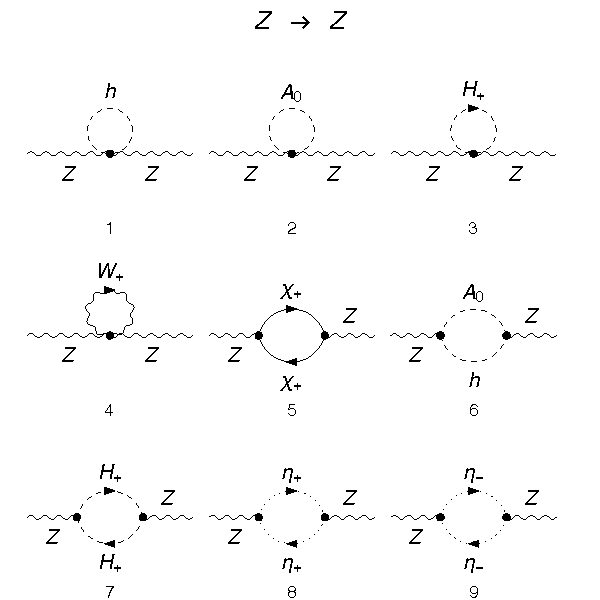
\includegraphics[width=0.5\textwidth]{diagrams_V[2]_1_1.pdf}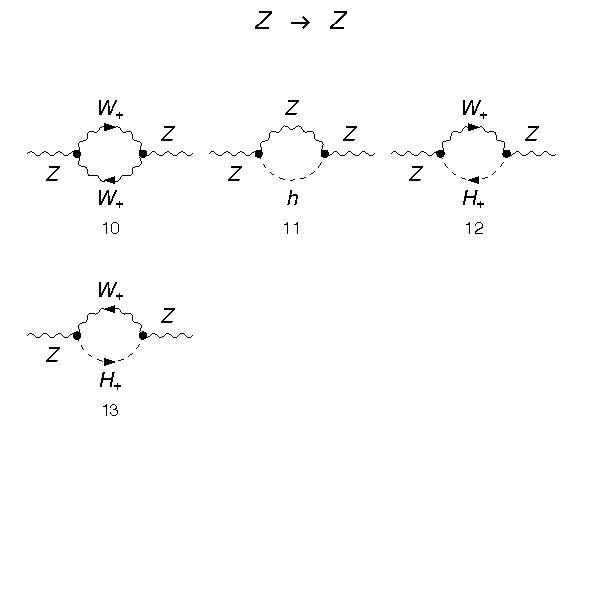
\includegraphics[width=0.5\textwidth]{diagrams_V[2]_1_2.pdf}
\caption{The one-loop corrections to the Z boson propagator.}\label{fig:gammagamma}
\end{figure}

\subsection{Z boson self energy}

The Z boson self energy as given by Ibe et al. is
{
\begin{eqnarray}
\Pi_{ZZ}^{(V,h)}(p^2) &=& 
-\frac{ \hat{g}^2 (12\hat{c}_W^4 - 4\hat{c}_W^2 + 1) }{16\pi^2 \hat{c}_W^2}
\tilde B_{22}(p^2, \hat{m}_W^2, \hat{m}_W^2) 
-\frac{ \hat{g}^2 \hat{c}_W^2 p^2 }{24\pi^2} \nonumber \\
&& -\frac{2\hat{g}^2}{16\pi^2}(2\hat{c}_W^2 p^2 + 2\hat{m}_W^2 - \hat{m}_Z^2)
B_0(p^2, \hat{m}_W^2, \hat{m}_W^2) \nonumber \\
&& -\frac{ \hat{g}^2 }{16\pi^2 \hat{c}_W^2}
[\tilde B_{22}(p^2, \hat{m}_Z^2, \hat{m}_h^2)
-\hat{m}_Z^2 B_0(p^2, \hat{m}_Z^2, \hat{m}_h^2) ]\\
\end{eqnarray}
}
which we compare with the FeynCalc calculation and corresponding reduction which gives us

{
\begin{eqnarray}
\Pi_{ZZ}^{(V,h)}(p^2) &=& 
-\frac{ \hat{g}^2} {576 c_W^4 p^2 \pi^2}\left\{
2 p^2 \left[-3 m_H^2 (-1 + s_W^2) + 2 p^2 (1 - 3 s_W^2 + 2 s_W^4) \right. \right.\nonumber\\
&& \left.+ 3 m_W^2 (19 - 58 s_W^2 + 64 s_W^4 - 24 s_W^6)\right] \nonumber\\
&&- 3 (m_W^2 + m_H^2 (-1 + s_W^2) - 2 p^2 (-1 + s_W^2)) A0\left(m_H^2\right)  \nonumber\\
 &&  + 12 p^2 (-9 + 29 s_W^2 - 32 s_W^4 + 12 s_W^6) A_0\left(m_W^2\right)  \nonumber\\
   && +3 ((m_W^2 + mh^2 (-1 + s_W^2) + 2 p^2 (-1 + s_W^2)) A0\left(m_Z^2\right)  \nonumber\\
   &&+ \left[-m_W^2 (m_Z^2 + 10 p^2) + mh^4 (-1 + s_W^2)\right.  \nonumber\\
   && \left. +     p^4 (-1 + s_W^2) + 2 mh^2 (m_W^2 - p^2 (-1 + s_W^2))\right] B_0\left(p^2, m_H^2, m_Z^2\right)  \nonumber\\
&&   -    p^2 (-1 + s_W^2) \left[4 mw^2 (15 - 32 s_W^2 + 12 s_W^4)\right.  \nonumber\\
&&  \left.      \left. +  p^2 (39 - 76 s_W^2 + 36 s_W^4)\right] B_0\left(p^2, m_W^2, m_W^2\right)))\right\}
\end{eqnarray}
}




\begin{figure}[h!]
\center
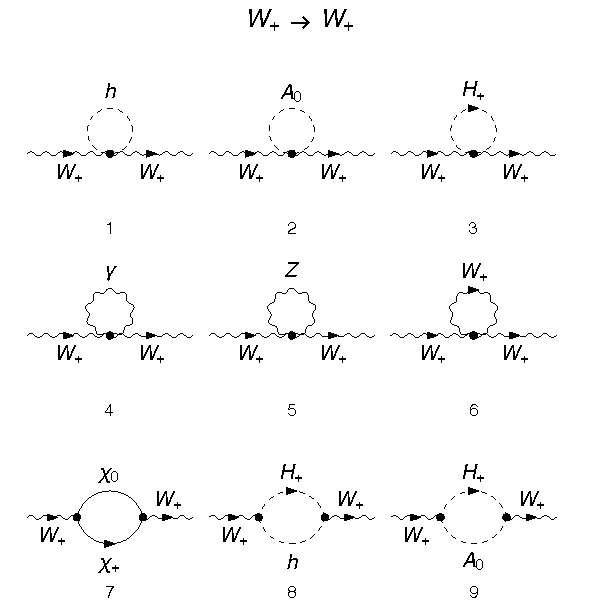
\includegraphics[width=0.5\textwidth]{diagrams_V[3]_1_1.pdf}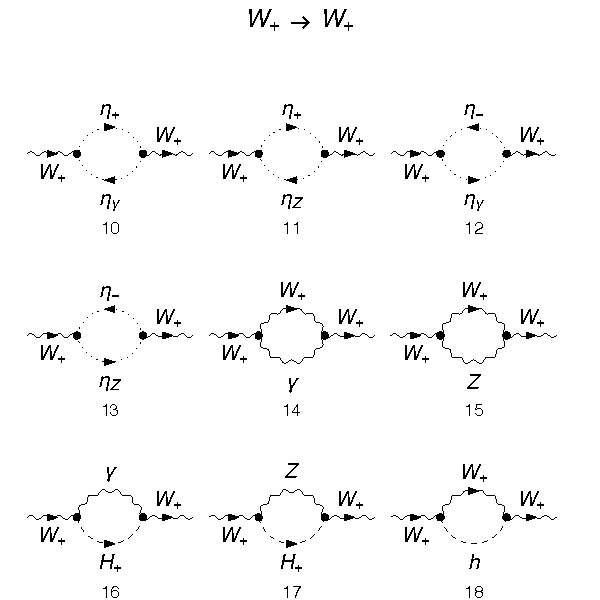
\includegraphics[width=0.5\textwidth]{diagrams_V[3]_1_2.pdf}
\caption{The one-loop corrections to the W boson propagator.}\label{fig:gammagamma}
\end{figure}

\subsection{W boson self energy}


{\small
\begin{eqnarray}
\Pi_{WW}^{(V, h)}(p^2) &=&
-\frac{8\hat{e}^2}{16\pi^2} \tilde B_{22}(p^2, 0, \hat{m}_W^2)
-\frac{\hat{e}^2 p^2}{24\pi^2}
-\frac{4\hat{e}^2 p^2}{16\pi^2} B_0(p^2, 0, \hat{m}_W^2) \nonumber \\
&& -\frac{\hat{g}^2}{16\pi^2}(1 + 8\hat{c}_W^2)
\tilde{B}_{22}(p^2, \hat{m}_W^2, \hat{m}_Z^2)
-\frac{\hat{g}^2 \hat{c}_W^2 p^2}{24\pi^2} \nonumber \\
&& -\frac{\hat g^2}{16\pi^2}( 4 \hat c_W^2 p^2 + 3 \hat m_W^2 - \hat m_Z^2) B_0( p^2, \hat m_W^2, \hat m_Z^2) \nonumber\\
&& -\frac{\hat{g}^2}{16\pi^2}
[ \tilde{B}_{22}(p^2, \hat{m}_W^2, \hat{m}_h^2)
-\hat{m}_W^2 B_0(p^2, \hat{m}_W^2, \hat{m}_h^2) ]\ .\label{eq:vhloop2}
\end{eqnarray}
}

We compute the self energy using the Mass Builder set up and find a consistent result if $m_{\gamma}=0$.  Before setting $m_{\gamma}=0$ we find obtain an additional term:

\begin{align}
\frac{g_2^2 m_{\gamma}^2 s_W^2 B_0(p^2,m_{\gamma}^2,m_W^2)}{16 \pi^2} = 0
\end{align}
for $m_{\gamma}=0$.  This is the only ``descrepancy" between our working and that of Ibe et al. where they have clearly just set this term to zero (as they do not explicitly use a  $m_{\gamma}$ quantity in their expressions, instead just using a zero).


{
\begin{eqnarray}
\Pi_{ZZ}^{(V,h)}(p^2) &=& 
-\frac{ \hat{g}^2} {576 c_W^4 p^2 \pi^2}\left\{ -6 mh^2 p^2 - 4 p^4 \right.\nonumber \\
&&+  24 (ma^2 - mw^2 - 2 p^2) s_W^2 (-1 + s_W^2) A0[ma^2] -  \nonumber\\
&&   3 mh^2 A0[mh^2] + 6 p^2 A0[mh^2] + 3 mh^2 A0[mw^2] +\nonumber \\
&&   60 p^2 A0[mw^2] + 54 p^2 A0[mz^2] + 3 mh^4 B0[p^2, mh^2, mw^2] -\nonumber \\
&&6 mh^2 p^2 B0[p^2, mh^2, mw^2] + 3 p^4 B0[p^2, mh^2, mw^2] + \nonumber\\
&&   3 mw^4 (B0[p^2, mh^2, mw^2] - B0[p^2, mw^2, mz^2])\nonumber \\
&&   + 3 mw^2 mz^2 B0[p^2, mw^2, mz^2] - 117 p^4 B0[p^2, mw^2, mz^2] \nonumber\\
&&   + 24 mw^4 s_W^4 (-B0[p^2, ma^2, mw^2] + B0[p^2, mw^2, mz^2])\nonumber \\
&&   + 24 mw^2 s_W^4 (A0[mz^2] + 2 (ma^2 + p^2) B0[p^2, ma^2, mw^2] - 2 p^2 B0[p^2, mw^2, mz^2])\nonumber \\
&&   - 12 s_W^4 \left[    2 ma^2 A0[mw^2] -  4 p^2 (ma^2 + A0[mz^2]) \right.\nonumber \\
&& \left. + (2 ma^4 - 7 ma^2 p^2 - 10 p^4) B0[p^2,ma^2, mw^2] + 10 p^4 B0[p^2, mw^2, mz^2]\right] \nonumber\\
&&  + mw^4 s_W^2 (24 B0[p^2, ma^2, mw^2] - 3 (B0[p^2, mh^2, mw^2] + B0[p^2, mw^2, mz^2])) \nonumber\\
&&   +  s_W^2 \left[-48 ma^2 p^2 + 6 mh^2 p^2 + 4 p^4 +  3 (mh^2 - 2 p^2) A0[mh^2] \right.\nonumber\\
&&   +  3 (8 ma^2 - mh^2 - 20 p^2) A0[mw^2] +\nonumber \\
&&      24 ma^4 B0[p^2, ma^2, mw^2] - 3 mh^4 B0[p^2, mh^2, mw^2] - \nonumber\\
&&    3 p^2 (34 A0[mz^2] + 4 (7 ma^2 + 10 p^2) B0[p^2, ma^2, mw^2] + (-2 mh^2 + p^2) B0[p^2, mh^2, mw^2] \nonumber\\
&& \left.- 79 p^2 B0[p^2, mw^2, mz^2])\right]    \nonumber\\
&& +  3 mw^2 (A0[mh^2] - A0[mw^2] \nonumber\\
&& -  2 ((mh^2 - 5 p^2) B0[p^2, mh^2, mw^2]\nonumber\\
&&       + p^2 (19 + 30 B0[p^2, mw^2, mz^2])))\nonumber \\
&&     - 3 mw^2 s_W^2 \left[A0[mh^2] - 2 A0[mw^2] + 9 A0[mz^2] + 2 (8 (ma^2 + p^2) B0[p^2, ma^2, mw^2] \right.\nonumber\\
&& \left. \left .- (mh^2 - 5 p^2) B0[p^2, mh^2, mw^2] - p^2 (18 + 43 B0[p^2, mw^2, mz^2]))\right] \right\}\nonumber
\end{eqnarray}
}





\subsection{Electroweak triplet self energies}
\textcolor{red}{The following is direct copy from Ibe et al.  need to restructure}

For the neutral wino, the amplitudes are given by
{
\begin{eqnarray}
\Sigma_{K, 0}^{(1)} &=&
-\frac{\hat{g}^2}{16\pi^2}
\left[ 4 B_1(p^2, \hat{M}_2^2, \hat{m}_W^2) + 2 \right]
+\delta_{Z_{\tilde{\chi}}}\ , \label{eq: Neu_K} \\
%%%%%
\Sigma_{M, 0}^{(1)} &=&
-\frac{\hat{g}^2 \hat{M}_2}{16\pi^2}
\left[ 8 B_0(p^2, \hat{M}_2^2, \hat{m}_W^2) - 4 \right]
-\delta_{M_{\tilde{\chi}}}\ . \label{eq: Neu_M}
\end{eqnarray}
}On the other hand, the two amplitudes for the charged wino are given by
{
\begin{eqnarray}
\Sigma_{K, \pm}^{(1)} =
-\frac{\hat{g}^2}{8\pi^2}
\left[ \hat{s}_W^2 B_1(p^2,\hat{M}_2^2,0)
+\hat{c}_W^2 B_1(p^2,\hat{M}_2^2, \hat m_Z^2)
+B_1(p^2, \hat{M}_2^2, \hat{m}_W^2) + 1  \right]
+ \delta_{Z_{\tilde{\chi}}}\ , \label{eq: Cha_K} \\
%%%%%
\Sigma_{M, \pm}^{(1)} =
-\frac{\hat{g}^2 \hat{M}_2}{4\pi^2}
\left[ \hat{s}_W^2 B_0(p^2, \hat{M}_2^2,0)
+\hat{c}_W^2 B_0(p^2, \hat{M}_2^2, \hat{m}_Z^2)
+B_0(p^2, \hat{M}_2^2, \hat{m}_W^2) - 1 \right]
-\delta_{M_{\tilde{\chi}}}\ ,
 \label{eq: Cha_M}
\end{eqnarray}
}where explicit forms of the counter-terms, $\delta_{Z_{\tilde{\chi}}}$ and $\delta_{M_{\tilde{\chi}}}$, are given in the following section.

Using Mass Builder we calculate the self energy in terms of $A_0$ and $B_0$ integrals exclusively.



\subsection{Calculation in Mass Builder}

We compute the gauge boson self energies and interface the output to TSIL automatically in Mass Builder.  This enables numerical calculation of the 1-loop self energies.  Using the input values and relationships in Table \ref{table:input_params} we calculate a one-loop pole mass of $(m_W^{(1)},m_Z^{(1)}) = ( , )$ GeV.

In our choice of gauge the ghost fields take on the same mass as their respective field, such that $m_{\eta_{\gamma}} = m_{\gamma}$, $m_{\eta_Z}=m_{Z}$, $m_{\eta^+}=m_{W}$.  The fields $A_0$ and $H^+$ from the pre-EWSB theory are also given the respective masses of $m_{A_0}=m_Z$ and $m_{H^+}=m_W$.


\begin{table}[tp]
\caption{The parameter values used for the electroweak triplet self energy calculations.  Where a derived quantity is used this is passed directly to Mass Builder in the analytic form. FIX THIS TABLE $Q=100$ ?!?!?}\label{table:input_params}
\centering
\begin{tabular}{l l}
\hline
Parameter & value\\
\hline
$m_W$ & $80.385$ GeV \\
$m_Z$ & $91.1876$ GeV \\
$v$ & 246 GeV \\
$Q$ & 100 \\
$c_W^2$ & $m^2_W/m^2_Z$ \\
$s_W^2$ & $1-c^2_W$ \\
$g_2$ & $2m_W/v$\\
$g_1$ & $g_2 s_W/c_W$\\
$m_H$ & 125.6 GeV\\
$M$ & 100 GeV\\
$m_{\gamma}$ & 0 \\
\hline\end{tabular}
\hspace{3cm}
\begin{tabular}{l l}
\hline
Field & 1-loop self energy (GeV)\\
\hline
$W$ & $-22649.4$ \\
$Z$ & $-17420.9$  \\
$\gamma$ & -4618.28 \\
$\chi^+$ & $20.0051$ \\
$\chi^0$ & $19.9978$ \\
&\\
\hline
Field & Physical mass (GeV)\\
\hline
$W$ & $80.5107$ \\
$Z$ & $91.169$  \\
$\gamma$ & $6.99911\times 10^{-8}$\\
\hline\end{tabular}
\end{table}

\subsection{1-loop counter-terms in Mass Builder}

We determine the one-loop counter-term couplings using the inbuilt Mass Builder feature.  After all diagrams have been computed, Mass Builder collects all amplitudes together and extracts the coefficient of $1/\epsilon$ and simplifies this give the one-loop counter term coupling.  It also prints out the coefficients of $1/\epsilon^2$ and $1/\epsilon^3$ as a check that higher order divergences do not exist.  With this method we determine the following counter-terms


\begin{eqnarray}
\delta_{Z_{WW}} &=&- \frac{g_2^2}{16 \pi^2}\left(-\frac{11}{6}\right),\\
\delta_{m^2_{WW}}&=&- \frac{g_2^2}{16 \pi^2} \left( m^2_Z(-1+2s_W^2)     -m_{\gamma}^2s_W^2\right),\\
\delta_{Z_{\gamma\gamma}} &=&-\frac{g_2^2s_W^2}{16 \pi^2}\left(-\frac{5}{3}\right) = \frac{\hat{e}^2}{16\pi^2}\left(-\frac{5}{3}\right) , \\
%%%%%
\delta_{m^2_{\gamma\gamma}} &=& 0\, ,\\
\delta_{Z_{ZZ}} &=&-\frac{g_2^2}{16 \pi^2 c_W^2} \left(-\frac{11}{6}+\frac{11}{3}s_W^2-\frac{5}{3}s_W^4  \right),\\
\delta_{m^2_{ZZ}} &=& -\frac{g_2^2m_Z^2}{16 \pi^2c_W^2} \left(-1+6s_W^2-4s_W^4  \right),\\
\delta_{m^2_{Z\gamma}} &=& -\frac{g_2^2s_W}{16 \pi^2c_W} \left( m_Z^2(2-2s_W^2)  \right),\\
\delta_{Z_{Z\gamma}} &=& -\frac{g_2^2s_W}{16 \pi^2c_W} \left( \frac{11}{6}-\frac{5s_W^2}{3}  \right)
\end{eqnarray}

These match those of Ibe et al. (if we neglect the terms which obviously come from the SM fermionic and leptonic interactions) for the case of $m_{\gamma}=0$.

As there is mixing between the Z boson and the photon also computed a counter-term coupling for the two point propagator $Z\rightarrow\gamma$.  This calculation is fully supported in \mb by using the additional \lstinline{-q} flag.

We also compute the one-loop counter-term couplings for the fermionic triplet
\begin{eqnarray}
\delta_{Z_{\chi^0\chi^0}} &=&-\frac{g_2^2}{8 \pi^2}\\
\delta_{M_{\chi^0\chi^0}} &=&-\frac{g_2^2 M}{2 \pi^2}
\end{eqnarray}
which agree with that of Ibe et al.

Finally, we also need the counter term for the $W\chi\chi$ interaction which we use the value from Ibe et al.
\begin{align}
\delta_{\chi\chi W} = \frac{g^3}{4 \pi^2}.
\end{align}

\subsection{2-loop self energy}

We are finally ready to compute the two-loop self energies for the electroweak triplet.  For the neutral (charged) component there are 48 (75) two-loop diagrams and eight (10) two-loop order counter-term diagrams.  


\begin{figure}[h!]
\center
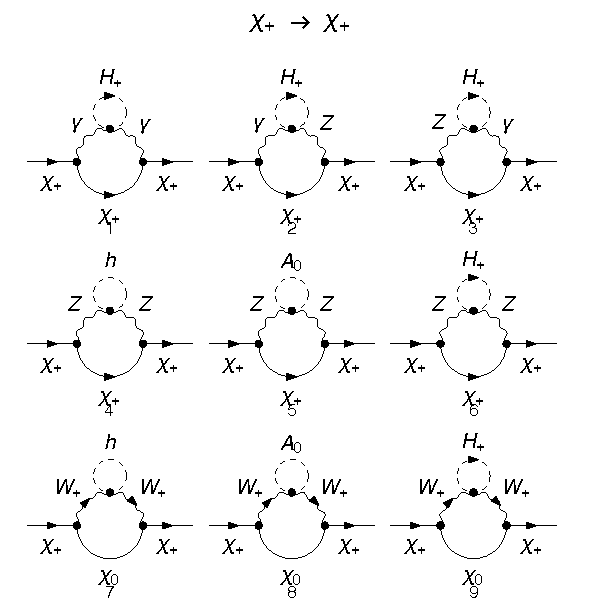
\includegraphics[width=0.5\textwidth]{diagrams_F[1]_2_1.pdf}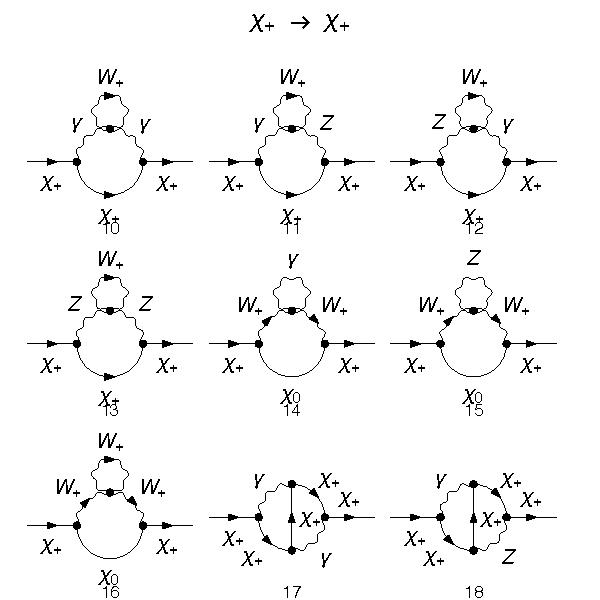
\includegraphics[width=0.5\textwidth]{diagrams_F[1]_2_2.pdf}
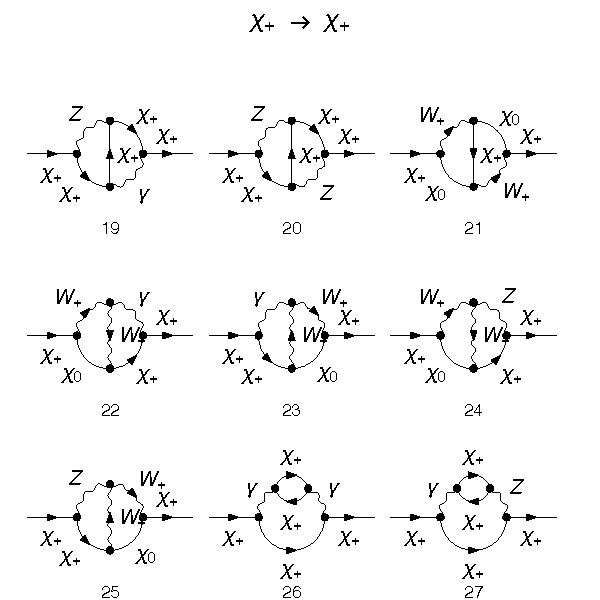
\includegraphics[width=0.5\textwidth]{diagrams_F[1]_2_3.pdf}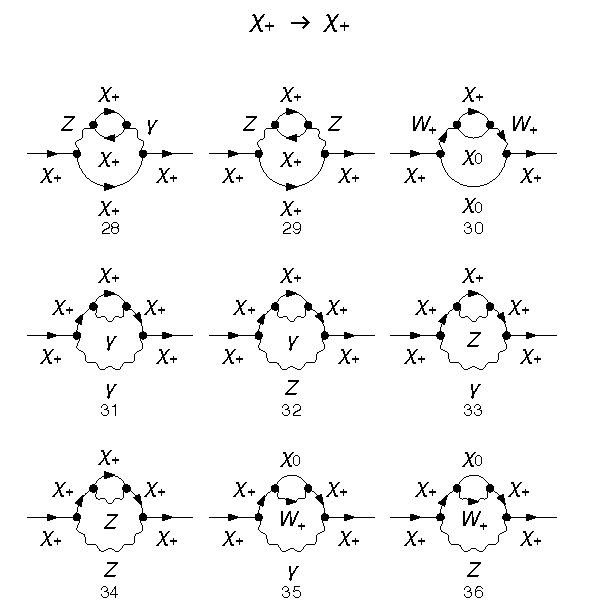
\includegraphics[width=0.5\textwidth]{diagrams_F[1]_2_4.pdf}
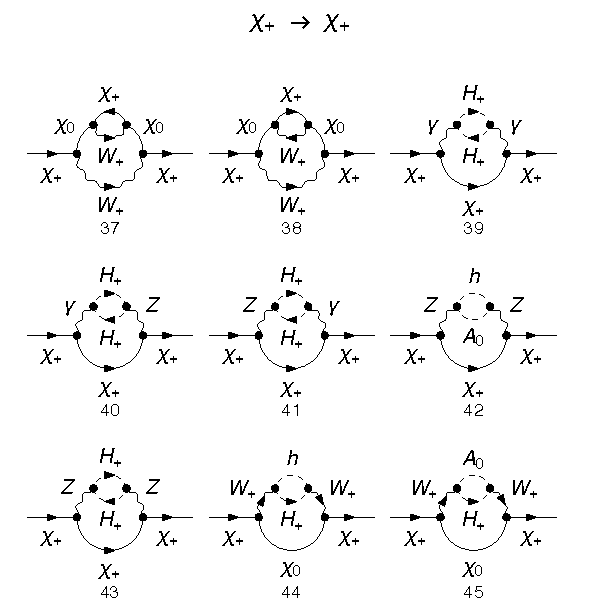
\includegraphics[width=0.5\textwidth]{diagrams_F[1]_2_5.pdf}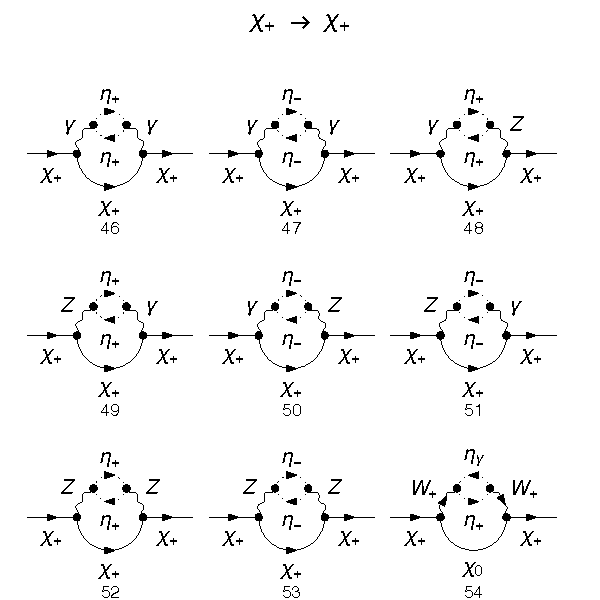
\includegraphics[width=0.5\textwidth]{diagrams_F[1]_2_6.pdf}
\caption{The two-loop corrections to the $\chi^+$ propagator.}\label{fig:chi1chi1_1}
\end{figure}

\begin{figure}[h!]
\center
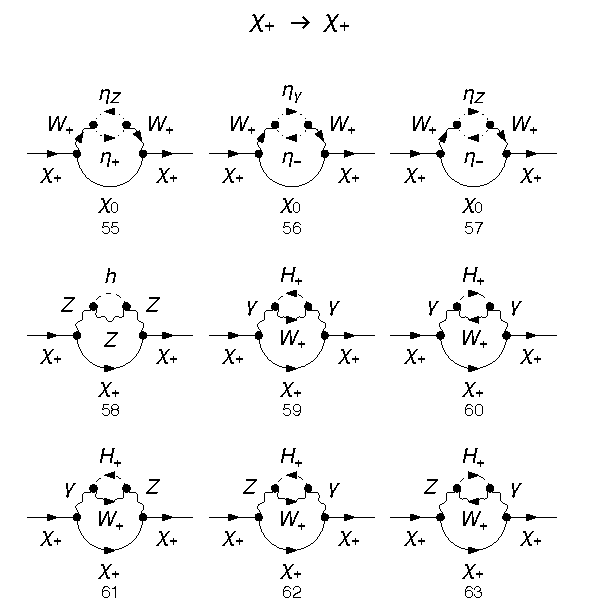
\includegraphics[width=0.5\textwidth]{diagrams_F[1]_2_7.pdf}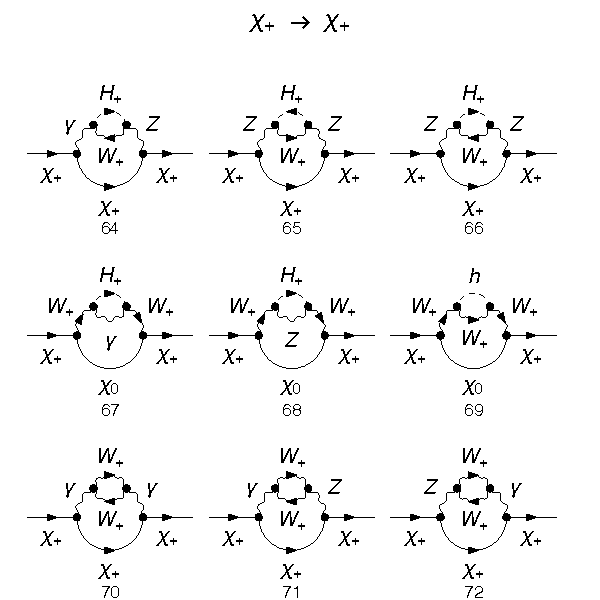
\includegraphics[width=0.5\textwidth]{diagrams_F[1]_2_8.pdf}
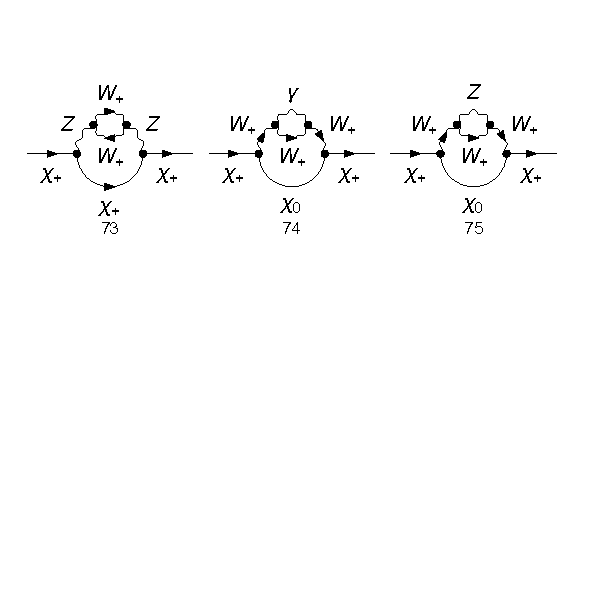
\includegraphics[width=0.5\textwidth]{diagrams_F[1]_2_9.pdf}
\caption{The two-loop corrections to the $\chi^+$ propagator.}\label{fig:chi1chi1_2}
\end{figure}

\begin{figure}[h!]
\center
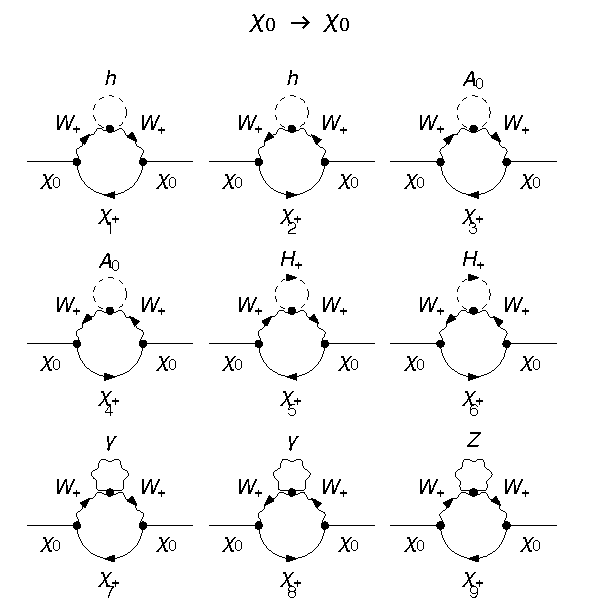
\includegraphics[width=0.5\textwidth]{diagrams_F[2]_2_1.pdf}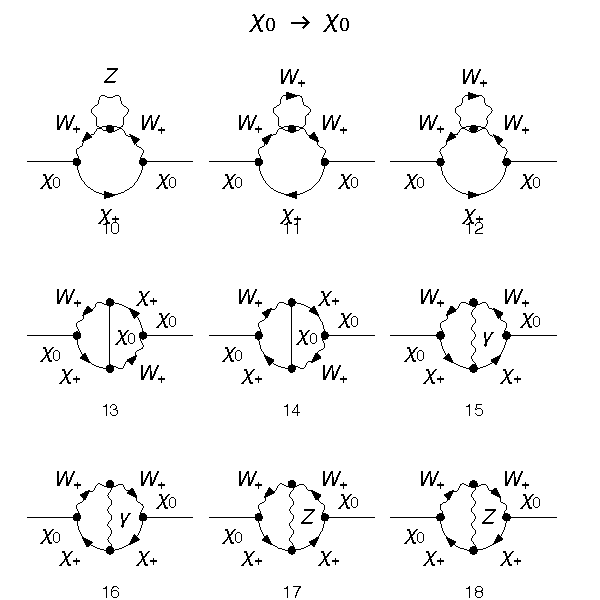
\includegraphics[width=0.5\textwidth]{diagrams_F[2]_2_2.pdf}
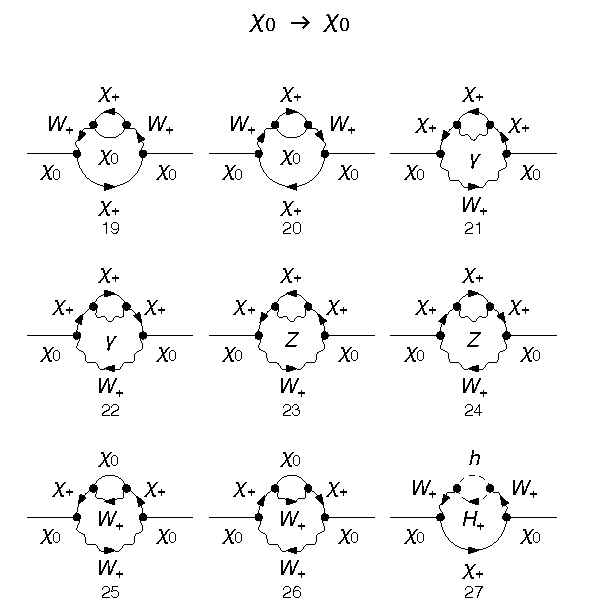
\includegraphics[width=0.5\textwidth]{diagrams_F[2]_2_3.pdf}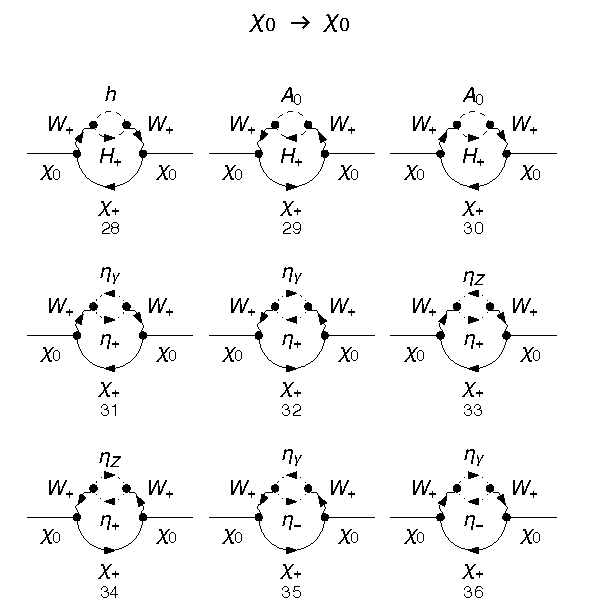
\includegraphics[width=0.5\textwidth]{diagrams_F[2]_2_4.pdf}
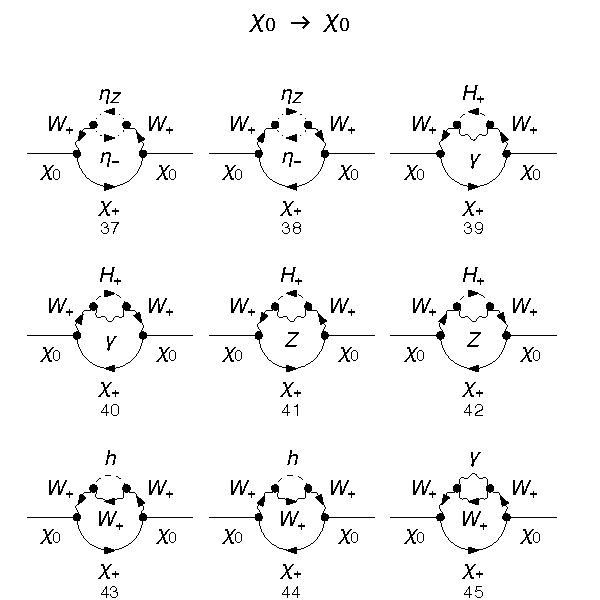
\includegraphics[width=0.5\textwidth]{diagrams_F[2]_2_5.pdf}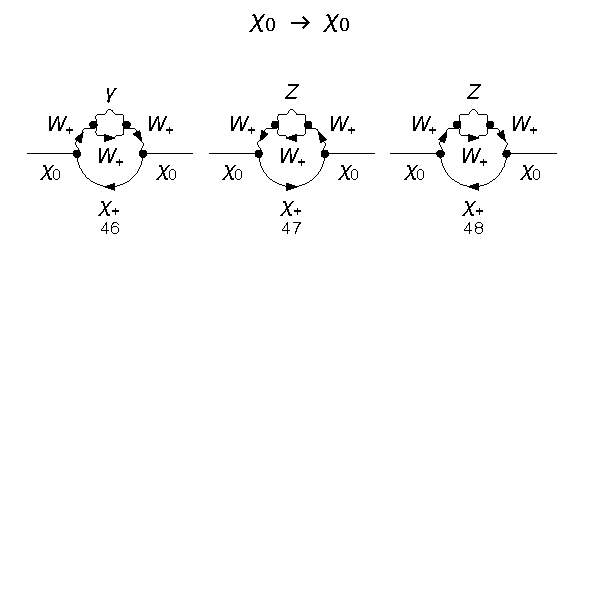
\includegraphics[width=0.5\textwidth]{diagrams_F[2]_2_6.pdf}
\caption{The two-loop corrections to the $\chi^0$ propagator.}\label{fig:chi0chi0}
\end{figure}



\begin{figure}[h!]
\center
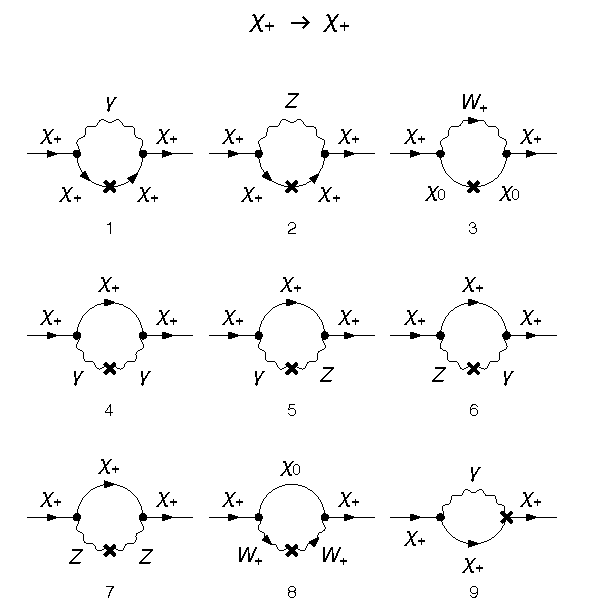
\includegraphics[width=0.5\textwidth]{diagrams_F[1]_2c_1.pdf}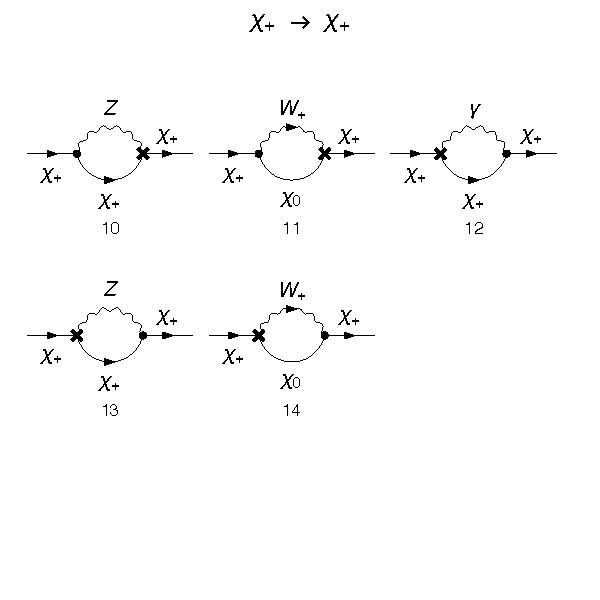
\includegraphics[width=0.5\textwidth]{diagrams_F[1]_2c_2.pdf}
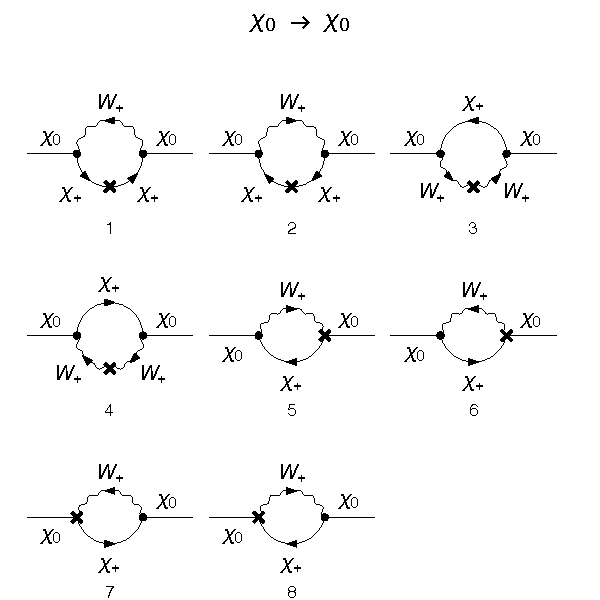
\includegraphics[width=0.5\textwidth]{diagrams_F[2]_2c.pdf}
\caption{The two-loop order counter-terms corrections to the $\chi^+$ and $\chi^0$ propagators.}\label{fig:chi_ct2}
\end{figure}

\end{document}  